% This is samplepaper.tex, a sample chapter demonstrating the
% LLNCS macro package for Springer Computer Science proceedings;
% Version 2.21 of 2022/01/12
%
\documentclass[runningheads]{llncs}
%
\usepackage[T1]{fontenc}
% T1 fonts will be used to generate the final print and online PDFs,
% so please use T1 fonts in your manuscript whenever possible.
% Other font encondings may result in incorrect characters.
%
\usepackage{graphicx}
\usepackage{menukeys}
\usepackage{xcolor,soul}
% Used for displaying a sample figure. If possible, figure files should
% be included in EPS format.
%
% If you use the hyperref package, please uncomment the following two lines
% to display URLs in blue roman font according to Springer's eBook style:
%\usepackage{color}
%\renewcommand\UrlFont{\color{blue}\rmfamily}
%\urlstyle{rm}
%
%% Enable non-ugly hyperlinks
\usepackage{blindtext}
\usepackage{epigraph}
\usepackage{multicol}

\usepackage{dsfont}
\usepackage{stmaryrd}
\usepackage{colortbl}
\usepackage{hyperref}

\usepackage{amsmath}
\DeclareMathOperator*{\argmax}{argmax}
\DeclareMathOperator*{\argmin}{argmin}
\usepackage{amssymb}

\usepackage[dvipsnames, table]{xcolor}
\usepackage{textcomp}

% Packages
\usepackage[pdf]{graphviz}
\usepackage{mathrsfs}

\newcommand*\circled[1]{\tikz[baseline=-0.1cm]{
  \node[shape=circle,draw,inner sep=0.48pt] (char) {\fontsize{7}{12}\textsf{#1}};}}

\DeclareMathAlphabet{\mathcal}{OMS}{cmsy}{m}{n}
\usepackage{cancel}
\newcommand\ccancel[2][red]{\renewcommand\CancelColor{\color{#1}}\cancel{#2}}
\newcommand{\nDownarrow}{\ensuremath{\text{ }\cancel{\Downarrow}\text{ }}}
\usepackage{centernot}

\usepackage{pgfplots, pgfplotstable}
\pgfplotsset{compat=1.7}
\usepgfplotslibrary{fillbetween}
\usetikzlibrary{patterns}
\pgfmathdeclarefunction{gauss}{2}{\pgfmathparse{1/(#2*sqrt(2*pi))*exp(-((x-#1)^2)/(2*#2^2))}}
\pgfmathdeclarefunction{nil}{1}{\pgfmathparse{0.001}}

\usepackage{arydshln}
\usepackage{adjustbox}
\usepackage{enumerate}
\usepackage{enumitem}
\usepackage{tikz-cd}
\usetikzlibrary{calc}
\usepackage{amsfonts}
%\usepackage{prooftrees}
\usepackage{bussproofs}
\renewcommand{\sectionautorefname}{\S}
\renewcommand{\subsectionautorefname}{\S}
\usepackage{float}

\usepackage{tikz-3dplot}
\usetikzlibrary{3d}
\usetikzlibrary{calligraphy}
\newif\ifshowcellnumber
\showcellnumbertrue

\usepackage{algorithm}
\usepackage[noend]{algpseudocode}
\usepackage{algorithmicx}
\usepackage{sourcecodepro}
\usepackage{tikz-qtree}
\usepackage{amsthm}
\usepackage{bm}
\usetikzlibrary{bayesnet}
\usetikzlibrary{arrows}
\usepackage{subcaption}
\usetikzlibrary{backgrounds}
\usetikzlibrary{tikzmark}
\usetikzlibrary{hobby}

\usepackage{mwe}

\newcommand{\E}{\mathbb{E}}
\newcommand{\Var}{\mathrm{Var}}
\newcommand{\Cov}{\mathrm{Cov}}

\newcommand{\CompOrder}{\mathcal{O}}
\def\graphspace{\mathbf{G}}
\def\Uniform{\mbox{\rm Uniform}}
\def\Gaussian{\mbox{\rm Gaussian}}
\def\Bernoulli{\mbox{\rm Bernoulli}}
\def\Dirichlet{\mbox{\rm Dirichlet}}

\usepackage{mathtools}% superior to amsmath
\usepackage{tikz}
% Packages
\usepackage{listings}
\DeclareRobustCommand{\hlred}[1]{{\sethlcolor{pink}\hl{#1}}}
\usepackage{fontspec}

\setmonofont[Scale=0.8]{JetBrainsMono}[
  Contextuals={Alternate},
  Path=./font/,
  Extension = .ttf,
  UprightFont=*-Regular,
  BoldFont=*-Bold,
  ItalicFont=*-Italic,
  BoldItalicFont=*-BoldItalic
]

\usepackage[skins,breakable,listings]{tcolorbox}

\lstdefinelanguage{python}{
  comment=[l]{//},
  commentstyle={\color{gray}\ttfamily},
  emph={delegate, filter, firstOrNull, forEach, it, lazy, mapNotNull, println, repeat, assert, with, head, tail, len, return@},
  numberstyle=\noncopyable,
  identifierstyle=\color{black},
  keywords={abstract, actual, as, as?, break, by, class, companion, continue, data, do, dynamic, else, enum, expect, false, final, for, fun, get, if, import, in, infix, interface, internal, is, null, object, open, operator, override, package, private, public, return, sealed, set, super, suspend, this, throw, true, try, catch, typealias, val, var, vararg, when, where, while, tailrec, reified, from, import, def, yield, lambda, as, in, return, else, pass},
  keywordstyle={\bfseries},
  morecomment=[s]{/*}{*/},
  morestring=[b]",
  morestring=[s]{"""*}{*"""},
  ndkeywords={@Deprecated, @JvmField, @JvmName, @JvmOverloads, @JvmStatic, @JvmSynthetic, Array, Byte, Double, Float, Boolean, Int, Integer, Iterable, Long, Runnable, Short, String, int},
  ndkeywordstyle={\bfseries},
  sensitive=true,
  stringstyle={\ttfamily},
  literate={`}{{\char0}}1,
  escapeinside={(*@}{@*)}
}

\lstnewenvironment{smallpy}
{\lstset{
  basicstyle=\ttfamily\lst@ifdisplaystyle\footnotesize\fi,
  language=python
}}
{}

\lstdefinelanguage{tidy}{
  comment=[l]{//},
  commentstyle={\color{gray}\ttfamily},
  emph={|, ->, ---},
  emphstyle={\color{red}},
  identifierstyle=\color{black},
  keywords={\|, ->, ---},
  otherkeywords={|,->},
  morekeywords={|,->},
  keywordstyle={\color{blue}\bfseries},
  morecomment=[s]{/*}{*/},
  morestring=[b]",
  morestring=[s]{"""*}{*"""},
  ndkeywords={@Deprecated, @JvmField, @JvmName, @JvmOverloads, @JvmStatic, @JvmSynthetic, Array, Byte, Double, Float, Int, Integer, Iterable, Long, Runnable, Short, String},
  ndkeywordstyle={\color{orange}\bfseries},
  sensitive=true,
  stringstyle={\color{green}\ttfamily},
  literate={`}{{\char0}}1
}

%%%%%%%%%%%%%%%%%%%%%%%%%%%%%%%%%%%%%%%%%%%
%
% Color boxes
%
%%%%%%%%%%%%%%%%%%%%%%%%%%%%%%%%%%%%%%%%%%%

\tcbset{
  enhanced jigsaw,
  breakable,
  listing only,
%  boxsep=-1pt,
%  top=-1pt,
  bottom=0.1cm,
  right=0.5cm,
  overlay first={
    \node[black!50] (S) at (frame.south) {\Large\ding{34}};
    \draw[dashed,black!50] (frame.south west) -- (S) -- (frame.south east);
  },
  overlay middle={
    \node[black!50] (S) at (frame.south) {\Large\ding{34}};
    \draw[dashed,black!50] (frame.south west) -- (S) -- (frame.south east);
    \node[black!50] (S) at (frame.north) {\Large\ding{34}};
    \draw[dashed,black!50] (frame.north west) -- (S) -- (frame.north east);
  },
  overlay last={
    \node[black!50] (S) at (frame.north) {\Large\ding{34}};
    \draw[dashed,black!50] (frame.north west) -- (S) -- (frame.north east);
  },
  before={\par\vspace{5pt}},
  after={\par\vspace{\parskip}\noindent}
}

\definecolor{slightgray}{rgb}{0.90, 0.90, 0.90}

\usepackage{soul}
\makeatletter
\def\SOUL@hlpreamble{%
  \setul{}{3.0ex}%
  \let\SOUL@stcolor\SOUL@hlcolor%
  \SOUL@stpreamble%
}
\makeatother

\newcommand{\inline}[1]{%
  \begingroup%
  \sethlcolor{slightgray}%
  \hl{\ttfamily\footnotesize #1}%
  \endgroup
}

\newcommand{\tinline}[1]{%
  \begingroup%
  \sethlcolor{slightgray}%
  \hl{\ttfamily\tiny #1}%
  \endgroup
}

\newtcblisting{halftidyinput}[1][]{%
  left skip=0.7cm,
  left=0.35cm,
  width=6cm,
%  left=-0.01cm,
  top=-0.1cm,
  bottom=-0.35cm,
  listing options={
    language=tidy,
    basicstyle=\ttfamily\small,
%numberstyle=\footnotesize,
    showstringspaces=false,
    tabsize=2,
    breaklines=true,
    numbers=none,
    inputencoding=utf8,
    escapeinside={(*@}{@*)},
    #1
  },
  underlay unbroken and first={%
    \path[draw=none] (interior.north west) rectangle node[white]{\includegraphics[width=4mm]{../figures/tidyparse_logo.png}} ([xshift=-10mm,yshift=-7mm]interior.north west);
  }
}

\newtcblisting{wholetidyinput}[1][]{%
  left skip=0.7cm,
  left=0.35cm,
  top=0.1cm,
  middle=0mm,
  boxsep=0mm,
  listing options={
    language=tidy,
    basicstyle=\ttfamily\small,
%numberstyle=\footnotesize,
    showstringspaces=false,
    tabsize=2,
    breaklines=true,
    numbers=none,
    inputencoding=utf8,
    escapeinside={(*@}{@*)},
    #1
  },
  underlay unbroken and first={%
    \path[draw=none] (interior.north west) rectangle node[white]{\includegraphics[width=4mm]{../figures/tidyparse_logo.png}} ([xshift=-10mm,yshift=-9mm]interior.north west);
  }
}

\definecolor{A}{RGB}{6,150,104}
\definecolor{B}{RGB}{196,74,137}
\definecolor{C}{RGB}{117,237,133}
\definecolor{D}{RGB}{246,46,243}
\definecolor{E}{RGB}{89,162,12}
\definecolor{F}{RGB}{113,12,158}
\definecolor{G}{RGB}{191,205,142}
\definecolor{H}{RGB}{51,58,158}
\definecolor{I}{RGB}{244,212,3}
\definecolor{J}{RGB}{37,36,249}
\definecolor{K}{RGB}{253,165,71}
\definecolor{L}{RGB}{27,81,29}
\colorlet{LA}{A!30}
\colorlet{LB}{B!30}
\colorlet{LC}{C!30}
\colorlet{LD}{D!30}
\colorlet{LE}{E!30}
\colorlet{LF}{F!30}
\colorlet{LG}{G!30}
\colorlet{LH}{H!30}
\colorlet{LI}{I!30}
\colorlet{LJ}{J!30}
\colorlet{LK}{K!30}
\colorlet{LL}{L!30}
\newcommand{\hiliA}[1]{%
  \colorbox{LA}{$#1$}}
\newcommand{\hiliB}[1]{%
  \colorbox{LB}{$#1$}}
\newcommand{\hiliC}[1]{%
  \colorbox{LC}{$#1$}}
\newcommand{\hiliD}[1]{%
  \colorbox{LD}{$#1$}}
\newcommand{\hiliE}[1]{%
  \colorbox{LE}{$#1$}}
\newcommand{\hiliF}[1]{%
  \colorbox{LF}{$#1$}}
\newcommand{\hiliG}[1]{%
  \colorbox{LG}{$#1$}}
\newcommand{\hiliH}[1]{%
  \colorbox{LH}{$#1$}}
\newcommand{\hiliI}[1]{%
  \colorbox{LI}{$#1$}}
\newcommand{\hiliJ}[1]{%
  \colorbox{LJ}{$#1$}}
\newcommand{\hiliK}[1]{%
  \colorbox{LK}{$#1$}}
\newcommand{\hiliL}[1]{%
  \colorbox{LL}{$#1$}}
\newcommand{\highlight}[1]{%
  \colorbox{lgray}{$#1$}}
\colorlet{lred}{red!30}
\colorlet{lorange}{orange!30}
\colorlet{lgreen}{green!30}
\colorlet{lgray}{black!15}
\colorlet{dgray}{black!75}
\DeclareRobustCommand{\hlred}[1]{{\sethlcolor{lred}\hl{#1}}}
\DeclareRobustCommand{\hlorange}[1]{{\sethlcolor{lorange}\hl{#1}}}
\DeclareRobustCommand{\hlgreen}[1]{{\sethlcolor{lgreen}\hl{#1}}}
\DeclareRobustCommand{\hlgray}[1]{{\sethlcolor{lgray}\hl{#1}}}
\DeclareRobustCommand{\caret}[1]{{\sethlcolor{dgray}\textcolor{white}{\hl{#1}}}}

\usepackage{url}
\usepackage{qtree}

\usepackage{filecontents}
\usepackage{pstricks-add}
\usepackage{emoji}
\usepackage{alltt}
\usepackage{nicematrix}
\usepackage{graphicx}
\usepackage{ulem}
\usepackage{upquote}
\tikzstyle{every picture}+=[remember picture]
\usepackage{menukeys}
\pgfplotstableread[col sep=comma,]{timings_loc.csv}\loctimings
\pgfplotstableread[col sep=comma,]{timings_unloc.csv}\unloctimings

\makeatletter
\DeclareRobustCommand{\cev}[1]{%
    {\mathpalette\do@cev{#1}}%
}
\newcommand{\do@cev}[2]{%
  \vbox{\offinterlineskip
  \sbox\z@{$\m@th#1 x$}%
  \ialign{##\cr
  \hidewidth\reflectbox{$\m@th#1\vec{}\mkern4mu$}\hidewidth\cr
  \noalign{\kern-\ht\z@}
    $\m@th#1#2$\cr
  }%
  }%
}
\makeatother

\makeatletter
\DeclareRobustCommand{\pder}[1]{%
  \@ifnextchar\bgroup{\@pder{#1}}{\@pder{}{#1}}}
\newcommand{\@pder}[2]{\frac{\partial#1}{\partial#2}}
\makeatother

\newcommand{\shup}{\shortuparrow}
\newcommand{\shri}{\shortrightarrow}
\newcommand{\shur}{\shup\hspace{-5pt}\shri}

\makeatletter
\def\squigglyred{\bgroup \markoverwith{\textcolor{red}{\lower3\p@\hbox{\sixly \char58}}}\ULon}
\makeatother

\makeatletter
\def\squigglyblu{\bgroup \markoverwith{\textcolor{blue}{\lower3\p@\hbox{\sixly \char58}}}\ULon}
\makeatother

\makeatletter
\def\squigglyora{\bgroup \markoverwith{\textcolor{orange}{\lower3\p@\hbox{\sixly \char58}}}\ULon}
\makeatother

\newcommand{\err}[1]{\smash{\squigglyred{#1}{}}}
\newcommand{\erb}[1]{\smash{\squigglyblu{#1}{}}}
\newcommand{\ero}[1]{\smash{\squigglyora{#1}{}}}
\newcommand{\stirlingii}{\genfrac{\{}{\}}{0pt}{}}

%======== Arrows =========
\newcommand{\knightarrow}{
  \tikz{
    \fill (0pt,0pt) circle [radius = 1pt];
    \fill (0pt,6pt) circle [radius = 1pt];
    \fill (6pt,0pt) circle [radius = 1pt];
    \fill (6pt,6pt) circle [radius = 1pt];
    \fill (12pt,0pt) circle [radius = 1pt];
    \fill (12pt,6pt) circle [radius = 1pt];
    \fill (6pt,0pt) circle [radius = 1pt];
    \fill (12pt,0pt) circle [radius = 1pt];
    \draw [-to] (0pt,0pt) -- (12pt,6pt);
  }
}

\newcommand{\kingarrow}{
  \tikz{
    \fill (0pt,0pt) circle [radius = 1pt];
    \fill (6pt,0pt) circle [radius = 1pt];
    \fill (0pt,6pt) circle [radius = 1pt];
    \fill (6pt,6pt) circle [radius = 1pt];
    \draw [-to] (0pt,0pt) -- (6pt,6pt);
    \draw [-to] (0pt,0pt) -- (0pt,6pt);
    \draw [-to] (0pt,0pt) -- (6pt,0pt);
  }
}

\newcommand{\duparrow}{
  \tikz{
    \fill[white] (0pt,0pt) circle [radius = 1pt];
    \fill (6pt,0pt) circle [radius = 1pt];
    \fill (0pt,6pt) circle [radius = 1pt];
    \fill[white] (6pt,6pt) circle [radius = 1pt];
    \draw [-to] (6pt,0pt) -- (0pt,6pt);
  }
}

\newcommand{\drightarrow}{
  \tikz{
    \fill (0pt,0pt) circle [radius = 1pt];
    \fill (6pt,0pt) circle [radius = 1pt];
    \draw [-to] (0pt,0pt) -- (6pt,0pt);
  }
}

\newcommand{\ddiagarrow}{
  \tikz{
    \fill (0pt,0pt) circle [radius = 1pt];
    \fill (6pt,0pt) circle [radius = 1pt];
    \fill (0pt,6pt) circle [radius = 1pt];
    \fill (6pt,6pt) circle [radius = 1pt];
    \draw [-to] (0pt,0pt) -- (6pt,6pt);
  }
}

\newcommand{\knightkingarrow}{
  \tikz{
    \fill (0pt,0pt) circle [radius = 1pt];
    \fill (0pt,6pt) circle [radius = 1pt];
    \fill (6pt,0pt) circle [radius = 1pt];
    \fill (6pt,6pt) circle [radius = 1pt];
    \fill (12pt,0pt) circle [radius = 1pt];
    \fill (12pt,6pt) circle [radius = 1pt];
    \draw [-to] (0pt,0pt) -- (6pt,6pt);
    \draw [-to] (0pt,0pt) -- (0pt,6pt);
    \draw [-to] (0pt,0pt) -- (6pt,0pt);
    \draw [-to] (0pt,0pt) -- (12pt,6pt);
  }
}

%======== Arrows =========

\usetikzlibrary{decorations.pathreplacing,automata,calc,positioning,matrix,chains,fit,decorations.pathmorphing}

\usepackage{wrapfig}

\newcommand{\mkTrellis}[1]{
  \begin{tikzpicture}
  \def\dx{20pt}
  \def\dy{30pt}
  \newcounter{i}
  \stepcounter{i}
  \node[circle, draw, fill=black!30] (\arabic{i}) at (0,0){};
  \foreach [count=\i] \x in {2,...,#1}{
    \pgfmathsetmacro{\lox}{\x-1}%
    \pgfmathsetmacro{\loxt}{\x-3}%
    \foreach [count=\j] \xx in {-\lox,-\loxt,...,\lox}{
      \pgfmathsetmacro{\jj}{\j-1}%
      \stepcounter{i}
      \pgfmathsetmacro{\kk}{\xx-2}%
      \pgfmathsetmacro{\lbl}{\lox!/(\jj!*(\lox-\jj)!)}
      \ifnum\x<\kk
      \pgfmath\node[circle, draw]  (\arabic{i}) at (\xx*\dx, -\lox*\dy) {};
      \else
        \pgfmath\node[circle, draw, fill=black!30]  (\arabic{i}) at (\xx*\dx, -\lox*\dy) {};
      \fi
    }
  }
  \newcounter{z}
  \newcounter{xn}
  \newcounter{xnn}
  \pgfmathsetmacro{\maxx}{#1 - 1}
  \foreach \x in {1,...,\maxx}{
    \foreach \xx in {1,...,\x}{
      \stepcounter{z}
      \setcounter{xn}{\arabic{z}}
      \addtocounter{xn}{\x}
      \setcounter{xnn}{\arabic{xn}}
      \stepcounter{xnn}
      \draw [<-] (\arabic{z}) -- (\arabic{xn});
      \draw [<-] (\arabic{z}) -- (\arabic{xnn});
    }
  }
  \end{tikzpicture}
}

\newcommand{\dx}{20pt}
\newcommand{\dy}{30pt}
\newcounter{i}
\newcounter{z}
\newcounter{xn}
\newcounter{xnn}
\newcommand{\mkTrellisAppend}[1]{
  \begin{tikzpicture}
  \setcounter{i}{0}
  \setcounter{z}{0}
  \setcounter{xn}{0}
  \setcounter{xnn}{0}
  \stepcounter{i}
  \node[circle, draw] (\arabic{i}) at (0,0){};
  \foreach [count=\i] \x in {2,...,#1}{
    \pgfmathsetmacro{\lox}{\x-1}%
    \pgfmathsetmacro{\loxt}{\x-3}%
    \foreach [count=\j] \xx in {-\lox,-\loxt,...,\lox}{
      \pgfmathsetmacro{\jj}{\j-1}%
      \stepcounter{i}
      \pgfmathsetmacro{\kk}{\xx+2}%
      \pgfmathsetmacro{\lbl}{\lox!/(\jj!*(\lox-\jj)!)}
      \ifnum\x>\kk
      \pgfmath\node[circle, draw, fill=black!30]  (\arabic{i}) at (\xx*\dx, -\lox*\dy) {};
      \else
        \pgfmath\node[circle, draw]  (\arabic{i}) at (\xx*\dx, -\lox*\dy) {};
      \fi
    }
  }
  \pgfmathsetmacro{\maxx}{#1 - 1}
  \foreach \x in {1,...,\maxx}{
    \foreach \xx in {1,...,\x}{
      \stepcounter{z}
      \setcounter{xn}{\arabic{z}}
      \addtocounter{xn}{\x}
      \setcounter{xnn}{\arabic{xn}}
      \stepcounter{xnn}
      \draw [<-] (\arabic{z}) -- (\arabic{xn});
      \draw [<-] (\arabic{z}) -- (\arabic{xnn});
    }
  }
  \end{tikzpicture}
}

\newcommand{\mkTrellisInsert}[1]{
  \begin{tikzpicture}
  \setcounter{i}{0}
  \setcounter{z}{0}
  \setcounter{xn}{0}
  \setcounter{xnn}{0}
  \stepcounter{i}
  \node[circle, draw] (\arabic{i}) at (0,0){};
  \foreach [count=\i] \x in {2,...,#1}{
    \pgfmathsetmacro{\lox}{\x-1}%
    \pgfmathsetmacro{\loxt}{\x-3}%
    \foreach [count=\j] \xx in {-\lox,-\loxt,...,\lox}{
      \pgfmathsetmacro{\jj}{\j-1}%
      \stepcounter{i}
      \pgfmathsetmacro{\mp}{\xx+#1}%
      \pgfmathsetmacro{\mq}{\xx+\x}%
      \pgfmathsetmacro{\lbl}{\lox!/(\jj!*(\lox-\jj)!)}
      \ifnum\x>\mp
      \pgfmath\node[circle, draw, fill=black!30]  (\arabic{i}) at (\xx*\dx, -\lox*\dy) {};
      \else
        \ifnum#1<\mq
        \pgfmath\node[circle, draw, fill=black!30]  (\arabic{i}) at (\xx*\dx, -\lox*\dy) {};
        \else
          \pgfmath\node[circle, draw]  (\arabic{i}) at (\xx*\dx, -\lox*\dy) {};
        \fi
      \fi

    }
  }
  \pgfmathsetmacro{\maxx}{#1 - 1}
  \foreach \x in {1,...,\maxx}{
    \foreach \xx in {1,...,\x}{
      \stepcounter{z}
      \setcounter{xn}{\arabic{z}}
      \addtocounter{xn}{\x}
      \setcounter{xnn}{\arabic{xn}}
      \stepcounter{xnn}
      \draw [<-] (\arabic{z}) -- (\arabic{xn});
      \draw [<-] (\arabic{z}) -- (\arabic{xnn});
    }
  }
  \end{tikzpicture}
}

\usetikzlibrary{automata, positioning, arrows}

\newcommand{\nobarfrac}{\genfrac{}{}{0pt}{}}
\pgfplotstableread[col sep=comma,]{timings_loc.csv}\loctimings
\pgfplotstableread[col sep=comma,]{timings_unloc.csv}\unloctimings
\pgfplotstableread[col sep=comma,]{natural_errors.csv}\naturalerrors
\pgfplotstableread[col sep=comma,]{synthetic_errors.csv}\syntheticerrors

\usepackage[all,pdf]{xy}

\newcommand{\bs}{\blacksquare}
\newcommand{\ws}{\square}

\usepackage{multicol}
\usetikzlibrary{shapes.geometric, arrows}

\tikzstyle{startstop} = [rectangle, rounded corners,
minimum width=3cm,
minimum height=1cm,
thick,
text centered,
draw=none,
]

\tikzstyle{plain} = [
rectangle,
rounded corners,
minimum width=3.5cm,
minimum height=1cm,
thick,
text centered,
draw=black
]

\tikzstyle{io} = [trapezium,
trapezium stretches=true, % A later addition
thick,
trapezium left angle=70,
trapezium right angle=110,
minimum width=3cm,
minimum height=1cm, text centered,
draw=black, fill=blue!30]

\tikzstyle{io2} = [trapezium,
trapezium stretches=true, % A later addition
thick,
trapezium left angle=70,
trapezium right angle=110,
minimum width=3cm,
minimum height=1cm, text centered,
draw=black, fill=black!30]

\tikzstyle{process} = [rectangle,
minimum width=3.5cm,
minimum height=1cm,
thick,
text centered,
text width=4cm,
draw=black,
fill=orange!30]

\tikzstyle{decision} = [diamond,
minimum width=2.5cm,
minimum height=0.5cm,
thick,
text centered,
draw=black,
fill=green!30]
\tikzstyle{arrow} = [->,thick]

%\usetikzlibrary{external}
%\tikzexternalize[prefix=figures/]
\definecolor{green}{RGB}{0,128,0}
\definecolor{darkgray176}{RGB}{176,176,176}
\definecolor{darkviolet1270255}{RGB}{127,0,255}
\definecolor{deepskyblue3176236}{RGB}{3,176,236}
\definecolor{dodgerblue45123246}{RGB}{45,123,246}
\definecolor{lightgray204}{RGB}{204,204,204}
\definecolor{royalblue8762253}{RGB}{87,62,253}

\usepackage{sankey}

\usepackage{pgfplots}
\usepackage{array,multirow,graphicx}
\usepackage{arydshln}
\usepackage{tablefootnote} % for table footnotes

\colorlet{lred}{red!30}
\colorlet{lorange}{orange!30}
\colorlet{lgreen}{green!30}
\DeclareRobustCommand{\hlred}[1]{{\sethlcolor{lred}\hl{#1}}}
\DeclareRobustCommand{\hlorange}[1]{{\sethlcolor{lorange}\hl{#1}}}
\DeclareRobustCommand{\hlgreen}[1]{{\sethlcolor{lgreen}\hl{#1}}}

\usepackage{bussproofs}
\usepackage{ulem}


\makeatletter
\def\squigglyred{\bgroup \markoverwith{\textcolor{red}{\lower3\p@\hbox{\sixly \char58}}}\ULon}
\makeatother

\makeatletter
\def\squigglyblu{\bgroup \markoverwith{\textcolor{blue}{\lower3\p@\hbox{\sixly \char58}}}\ULon}
\makeatother

\makeatletter
\def\squigglyora{\bgroup \markoverwith{\textcolor{orange}{\lower3\p@\hbox{\sixly \char58}}}\ULon}
\makeatother

\newcommand{\err}[1]{\smash{\squigglyred{#1}{}}}
\newcommand{\erb}[1]{\smash{\squigglyblu{#1}{}}}
\newcommand{\ero}[1]{\smash{\squigglyora{#1}{}}}
\newcommand{\stirlingii}{\genfrac{\{}{\}}{0pt}{}}
\usepackage{amsmath,bm}
\usepackage{dsfont}
\DeclareMathOperator*{\argmax}{argmax}
\DeclareMathOperator*{\argmin}{argmin}
\usepackage{amssymb}% http://ctan.org/pkg/amssymb

\usepackage{hyperref}
\usepackage{pifont}% http://ctan.org/pkg/pifont
\newcommand{\cmark}{\ding{51}}%
\newcommand{\xmark}{\ding{55}}%
\usepackage{inconsolata}
\usepackage{tikz}
\usetikzlibrary{automata, positioning, arrows}

\usepackage{listings}
\usepackage[skins,breakable,listings]{tcolorbox}

%%%%%%%%%%%%%%%%%%%%%%%%%%%%%%%%%%%%%%%%%%%
%
% Color boxes
%
%%%%%%%%%%%%%%%%%%%%%%%%%%%%%%%%%%%%%%%%%%%

\tcbset{
  enhanced jigsaw,
  breakable,
  listing only,
%  boxsep=-1pt,
%  top=-1pt,
  width=0.9\textwidth,
  left=0.4cm,
  bottom=0cm,
  right=0cm,
  left skip=1.8cm,
  boxrule=1pt,
  overlay first={
    \node[black!50] (S) at (frame.south) {\Large\ding{34}};
    \draw[dashed,black!50] (frame.south west) -- (S) -- (frame.south east);
  },
  overlay middle={
    \node[black!50] (S) at (frame.south) {\Large\ding{34}};
    \draw[dashed,black!50] (frame.south west) -- (S) -- (frame.south east);
    \node[black!50] (S) at (frame.north) {\Large\ding{34}};
    \draw[dashed,black!50] (frame.north west) -- (S) -- (frame.north east);
  },
  overlay last={
    \node[black!50] (S) at (frame.north) {\Large\ding{34}};
    \draw[dashed,black!50] (frame.north west) -- (S) -- (frame.north east);
  },
  before={\par\vspace{5pt}},
  after={\par\vspace{\parskip}\noindent}
}

\definecolor{slightgray}{rgb}{0.90, 0.90, 0.90}

\usepackage{soul}
\makeatletter
\def\SOUL@hlpreamble{%
  \setul{}{3.0ex}%
  \let\SOUL@stcolor\SOUL@hlcolor%
  \SOUL@stpreamble%
}
\makeatother

\newcommand{\inline}[1]{%
  \begingroup%
  \sethlcolor{slightgray}%
  \hl{\ttfamily\footnotesize #1}%
  \endgroup
}

\newcommand{\tinline}[1]{%
  \begingroup%
  \sethlcolor{slightgray}%
  \hl{\ttfamily\tiny #1}%
  \endgroup
}

\newtcblisting{wholetidyinput}[1][]{%
  left=0.4cm,
  top=0.1cm,
%  width=0.9\textwidth,
  middle=0mm,
  boxsep=0mm,
  listing options={
    language=tidy,
    basicstyle=\ttfamily\scriptsize,
%numberstyle=\footnotesize,
    showstringspaces=false,
    tabsize=2,
    breaklines=true,
    numbers=none,
    inputencoding=utf8,
    escapeinside={(*@}{@*)},
    #1
  },
  underlay unbroken and first={%
    \path[draw=none] (interior.north west) rectangle node[white]{\includegraphics[width=4mm]{../figures/tidyparse_logo.png}} ([xshift=-10mm,yshift=-8mm]interior.north west);
  }
}

%\usepackage{sourcecodepro}
%\usepackage{newtxtt}
%\usepackage{zi4}
%\usepackage{FiraMono}
%\usepackage{DejaVuSansMono}

%\usepackage{fontspec}
%\setmonofont[Scale=0.8]{JetBrainsMono}[
%  Contextuals={Alternate},
%  Path=./font/,
%  Extension = .ttf,
%  UprightFont=*-Regular,
%  BoldFont=*-Bold,
%  ItalicFont=*-Italic,
%  BoldItalicFont=*-BoldItalic
%]

\definecolor{green}{RGB}{0,128,0}
\definecolor{darkgray176}{RGB}{176,176,176}
\definecolor{darkviolet1270255}{RGB}{127,0,255}
\definecolor{deepskyblue3176236}{RGB}{3,176,236}
\definecolor{dodgerblue45123246}{RGB}{45,123,246}
\definecolor{lightgray204}{RGB}{204,204,204}
\definecolor{royalblue8762253}{RGB}{87,62,253}

\begin{document}
%
\title{Tidyparse: A Tool for Realtime Syntax Repair}
%
\titlerunning{Tidyparse: A Tool for Realtime Syntax Repair}
% If the paper title is too long for the running head, you can set
% an abbreviated paper title here
%
\author{Breandan Considine\inst{1} \and
Jin Guo\inst{1}\and
Xujie Si\inst{2}}
%
\authorrunning{Considine et al.}
% First names are abbreviated in the running head.
% If there are more than two authors, 'et al.' is used.
%
\institute{McGill University, Montr\'eal, QC H2R 2Z4, Canada\\
\email{\{breandan.considine@mail, jguo@cs\}.mcgill.ca}\and
University of Toronto, Toronto, ON, M5S 1A1 Canada\\
\email{six@utoronto.ca}}
%
\maketitle              % typeset the header of the contribution
%
\begin{abstract}
  We describe the implementation of a tool for real-time syntax correction in an IDE. Upon activation, our tool takes a syntactically invalid source code fragment around the caret position, and produces a small set of suggested repairs. We model the problem of syntax repair as a structured prediction task, whose goal is to generate the most likely valid repair in a small edit distance of the invalid code fragment.
  \keywords{Error correction \and CFL reachability \and Language games.}
\end{abstract}

\section{Introduction}

Syntax errors are a familiar nuisance for software developers. Whenever a syntax error is detected, the IDE typically flags the offending code fragment, but offers little guidance on how it should be fixed. The developer must inspect the code and manually apply the appropriate fix through a process of trial and error. This process can be distracting and time-consuming, especially for novice developers. In this paper, we describe a tool for automatic syntax repair in an IDE.

We propose a new approach to syntax repair and accompanying tool, called \textit{Tidyparse} that suggests a small set of repairs to the user, which are guaranteed to be valid, minimal and natural. Our repair tool is a fusion of two widely available components: grammars and language models. At first glance, these two models are not obviously synergistic: the grammar is a deterministic, formal model of the language, while the language model is only an approximate generator of linguistic patterns. However, we show that by carefully integrating them, it is possible to generate repairs that are always correct and highly natural.

Language models are statistical models that generate natural sequences of text, however, these models make no guarantees about the validity of the generated text. Given a sequence of previous tokens, $\sigma_{0}, \ldots, \sigma_{n-1}$, an autoregressive language model outputs a distribution over the next most likely token, $\sigma_n$.

Almost every programming language ever developed is syntactically context-free, meaning the syntax of the language can be expressed as a context-free grammar (CFG). This grammar can be used to recognize the validity of a given input sequence, or force an autoregressive language model to generate only syntactically valid sequences by blocking out invalid tokens during inference.

Likewise, this grammar can be also used to construct a synthetic grammar, recognizing all and only valid sequences within a certain edit distance of a broken source code fragment. Our approach uses a pretrained language model to sample repair candidates from this synthetic grammar. We rank the results by negative log likelihood under the language model, and present the top $k$ candidates to the user. The user can then select the most appropriate repair from the list.

Let us consider a simplified example. Suppose the user has just written the following code fragment: \texttt{v = df.iloc(5:, 2:)}. Given an alphabet of just a few dozen lexical tokens, this tiny statement has millions of possible two-token edits, yet only six of those possibilities are accepted by the Python parser:\vspace{-0.3cm}

\begin{figure}[h!]
  \noindent\begin{tabular}{@{}l@{\hspace{10pt}}l@{\hspace{10pt}}l@{}}
  (1) \texttt{v = df.iloc(5\hlred{:}, 2\hlorange{,})} & (3) \texttt{v = df.iloc(5\hlgreen{[}:, 2:\hlgreen{]})} & (5) \texttt{v = df.iloc\hlorange{[}5:, 2:\hlorange{]}} \\
  \rule{0pt}{4ex}(2) \texttt{v = df.iloc(5\hlorange{)}, 2\hlorange{(})} & (4) \texttt{v = df.iloc(5\hlred{:}, 2\hlred{:})} & (6) \texttt{v = df.iloc(5\hlgreen{[}:, 2\hlorange{]})}\\
  \end{tabular}\vspace{-5pt}
\end{figure}

\vspace{-0.3cm}\noindent The color \hlgreen{green} denotes an insertion, \hlorange{orange} is substitution and \hlred{red} is deletion. To generate these repairs, we start by lexicalizing the input sequence as follows:

\begin{verbatim}
              v    = df   . iloc ( 5      : , 2      : )
              NAME = NAME . NAME ( NUMBER : , NUMBER : )
\end{verbatim}

\noindent Next, we construct an automaton that recognizes every string within a certain edit distance of the input. We will depict this process for a simpler language, where the grammar is $S \rightarrow \texttt{( )} \mid \texttt{( } S \texttt{ )} \mid S S$ and the broken code is \texttt{( ) )}.\vspace{-0.3cm}

\begin{figure}[h!]
  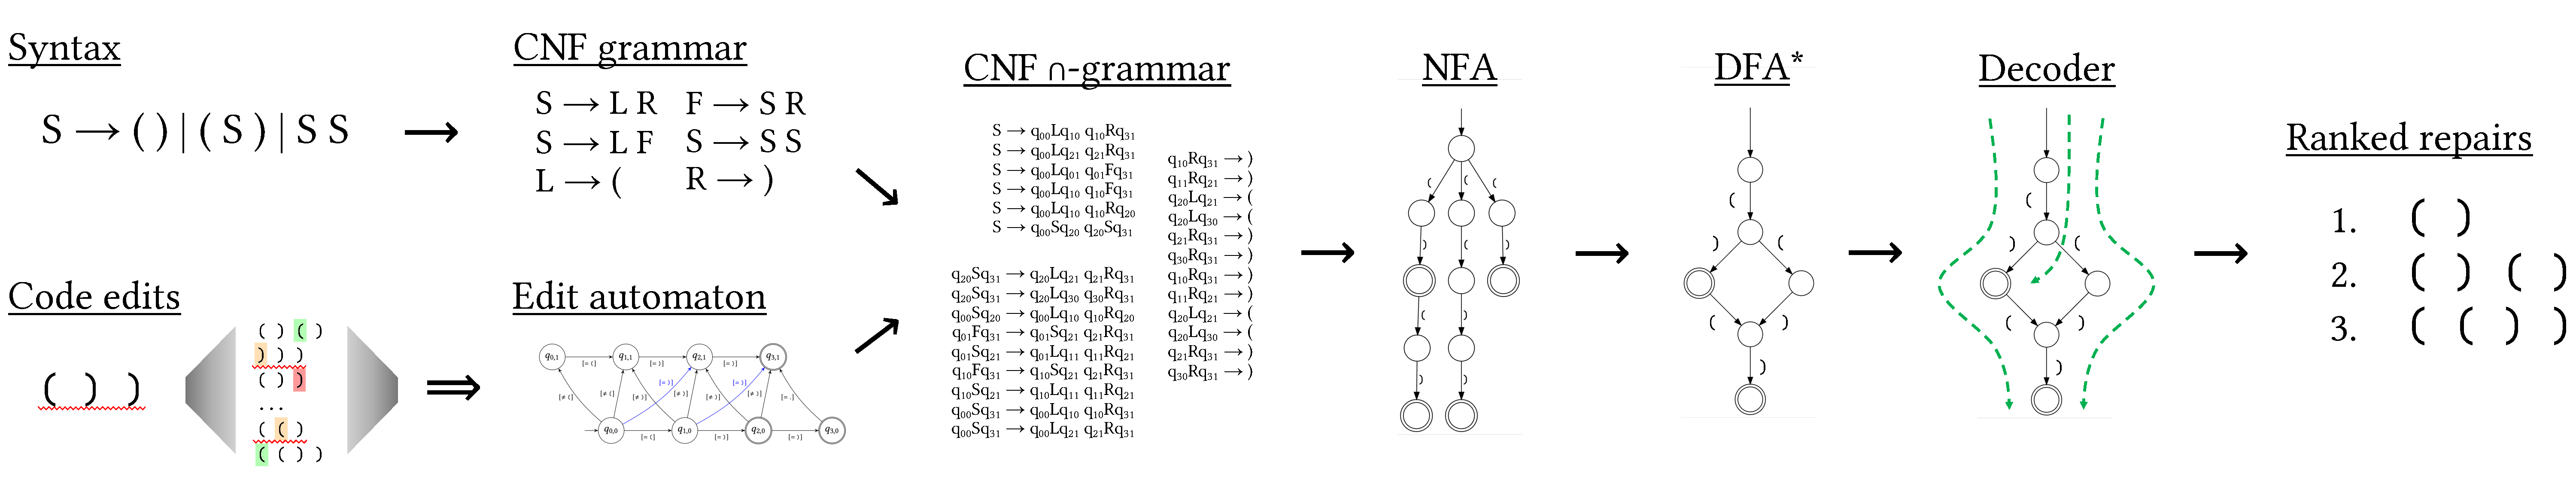
\includegraphics[width=\textwidth]{flow.pdf}\vspace{-1pt}
  \caption{Simplified dataflow. Given a grammar and broken code fragment, we create an automaton generating the language of small edits, then intersect it with the grammar to produce an intersection grammar, which can be simplified to a DFA and decoded.}\label{fig:arch_simp}
\end{figure}\vspace{-0.3cm}

The programming language syntax is represented by a context-free grammar, which we first reduce the grammar to Chomsky normal form (CNF). Then, using a modified construction from Bar-Hillel~\cite{bar1961formal}, we construct an intersection grammar, which recognizes all and only valid sequences recognized by both the grammar and edit automaton. This grammar is known to be non-recursive, and can be simplified to a deterministic finite automaton (DFA) using standard techniques. Finally, we decode the DFA to produce a list of repair candidates, which are reranked by a scoring function, e.g., the log likelihood of a language model.

Now that we have a high-level overview of our approach, we will demonstrate a few of the capabilities of our tool by means of some usage examples.

\section{Usage examples}

Tidyparse offers a convenient user interface featuring a text editor, a grammar editor and a parse tree viewer for interactive prototyping. All tokens are delimited by whitespace. For example, suppose we have the following grammar:

\begin{wholetidyinput}
  S -> S and S | S xor S | ( S ) | true | false | ! S(*@\caret{ }@*)
\end{wholetidyinput}

\noindent Syntax repair is the primary intended use case of our tool. If given an unparsable string, it will return an ordered set of suggestions how to fix it:

\begin{tcolorbox}[
top=0.1cm,
middle=0mm,
boxsep=0mm,
underlay unbroken and first={%
  \path[draw=none] (interior.north west) rectangle node[white]{\includegraphics[width=4mm]{../figures/tidyparse_logo.png}} ([xshift=-10mm,yshift=-9mm]interior.north west);
}]
\begin{lstlisting} [language=tidy, basicstyle=\ttfamily\scriptsize, escapeinside={(*@}{@*)}]
true and ( false or and true false(*@\caret{ }@*)
\end{lstlisting}
\tcblower
\begin{lstlisting} [language=tidy, basicstyle=\ttfamily\scriptsize, escapeinside={(*@}{@*)}]
1. true and ( false or (*@\hlorange{!}@*) true (*@\hlorange{)}@*)
2. true and ( false or (*@\hlgreen{<S>}@*) and true (*@\hlorange{)}@*)
3. true and ( false or (*@\hlorange{(}@*) true (*@\hlorange{)}@*) (*@\hlgreen{)}@*)
...
9. true and ( false or (*@\hlgreen{!}@*) (*@\hlgreen{<S>}@*) (*@\hlgreen{)}@*) and true (*@\hlred{false} @*)
\end{lstlisting}
\end{tcolorbox}
%Code completion is the secondary intended use case. Given a string containing a mixture of code and holes, our tool will return several possible completions:
%
%\begin{tcolorbox}[
%top=0.1cm,
%middle=0mm,
%boxsep=0mm,
%underlay unbroken and first={%
%  \path[draw=none] (interior.north west) rectangle node[white]{\includegraphics[width=4mm]{../figures/tidyparse_logo.png}} ([xshift=-10mm,yshift=-9mm]interior.north west);
%}]
%\begin{lstlisting} [language=tidy, basicstyle=\ttfamily\scriptsize, escapeinside={(*@}{@*)}]
%true _ _ _ ( false _ ( _ _ _ _ ! _ _ ) _ _ _ _(*@\caret{ }@*)
%\end{lstlisting}
%\tcblower
%\begin{lstlisting} [language=tidy, basicstyle=\ttfamily\scriptsize, escapeinside={(*@}{@*)}]
%1. true (*@\hlorange{xor}@*) (*@\hlorange{!}@*) ( false (*@\hlorange{xor}@*) ( (*@\hlorange{<S>}@*) (*@\hlorange{)}@*) (*@\hlorange{or}@*) ! (*@\hlorange{<S>}@*) ) (*@\hlorange{xor}@*) (*@\hlorange{<S>}@*)
%2. true (*@\hlorange{xor}@*) (*@\hlorange{!}@*) ( false (*@\hlorange{and}@*) ( (*@\hlorange{<S>}@*) (*@\hlorange{)}@*) (*@\hlorange{or}@*) ! (*@\hlorange{<S>}@*) ) (*@\hlorange{xor}@*) (*@\hlorange{<S>}@*)
%3. true (*@\hlorange{xor}@*) (*@\hlorange{!}@*) ( false (*@\hlorange{and}@*) ( (*@\hlorange{<S>}@*) (*@\hlorange{)}@*) (*@\hlorange{and}@*) ! (*@\hlorange{<S>}@*) ) (*@\hlorange{xor}@*) (*@\hlorange{<S>}@*)
%4. true (*@\hlorange{xor}@*) (*@\hlorange{!}@*) ( false (*@\hlorange{and}@*) ( (*@\hlorange{<S>}@*) (*@\hlorange{)}@*) (*@\hlorange{and}@*) ! (*@\hlorange{<S>}@*) ) (*@\hlorange{and}@*) (*@\hlorange{<S>}@*)
%...
%\end{lstlisting}
%\end{tcolorbox}
%
%

\vspace{-0.2cm}For simplicity, it is also possible to define a grammar and string side-by-side from the same editor, as shown in the untyped $\lambda$-calculus example below:

\begin{tcolorbox}[
top=0.1cm,
middle=0mm,
boxsep=0mm,
underlay unbroken and first={%
  \path[draw=none] (interior.north west) rectangle node[white]{\includegraphics[width=4mm]{../figures/tidyparse_logo.png}} ([xshift=-10mm,yshift=-9mm]interior.north west);
}]
\begin{lstlisting} [language=tidy, basicstyle=\ttfamily\scriptsize, escapeinside={(*@}{@*)}]
sxp -> (*@$\lambda$@*) var . sxp | sxp sxp | var | ( sxp )
var -> a | b | c | f | x | y | z
---
( (*@$\lambda$@*) f . ( (*@$\lambda$@*) x . f ( x x ) ) ( (*@$\lambda$@*) x . f ( x x ) (*@\caret{ }@*)
\end{lstlisting}
\tcblower
\begin{lstlisting} [language=tidy, basicstyle=\ttfamily\scriptsize, escapeinside={(*@}{@*)}]
1. ( (*@$\lambda$@*) f . ( (*@$\lambda$@*) x . f ( x x ) ) (*@\hlorange{)}@*) (*@$\lambda$@*) x . f ( x x )
2. ( (*@$\lambda$@*) f . ( (*@$\lambda$@*) x . f ( x x ) ) (*@\hlorange{x}@*) (*@\hlgreen{)}@*) (*@$\lambda$@*) x . f ( x x )
3. ( (*@$\lambda$@*) f . ( (*@$\lambda$@*) x . f ( x x ) ) ( (*@$\lambda$@*) x . f ( x(*@\hlred{ }@*)) (*@\hlgreen{)}@*) (*@\hlgreen{)}@*)
\end{lstlisting}
\end{tcolorbox}

\vspace{-0.2cm}\noindent By default, Tidyparse samples the finite intersection language uniformly without replacement, then sorts the results by Levenshtein distance. Customizing the ranking order is possible using a programmatic interface. For the Python language, we use a small dataset of n-grams to rank the repairs by naturalness.

%Since CFLs are closed under homomorphisms, it is possible to unify lexing and parsing, however most languages explicitly define a separate lexer, which we avail to substitute named identifiers with their type. Given an invalid string, the tool will first abstract the raw characters, generate edits in the abstract token space, then remap successful repairs back to character space as shown below:
%
%\hspace{-0.4cm}\begin{minipage}[t]{0.5\textwidth}
%                 \begin{tcolorbox}[
%                 left skip=0.7cm,
%                 left=0.35cm,
%                 width=0.9\textwidth,
%                 right=0cm,
%                 top=0.1cm,
%                 middle=0mm,
%                 boxsep=0mm,
%                 underlay unbroken and first={%
%                   \path[draw=none] (interior.north west) rectangle node[white]{\includegraphics[width=4mm]{../figures/tidyparse_logo.png}} ([xshift=-10mm,yshift=-9mm]interior.north west);
%                 }]
%                 \begin{lstlisting} [hbox, language=tidy, basicstyle=\ttfamily\scriptsize, escapeinside={(*@}{@*)}]
%d = sum([foo(i] for i in vals))(*@\caret{ }@*)
%                 \end{lstlisting}
%                 \tcblower
%                 \begin{lstlisting} [hbox, language=tidy, basicstyle=\ttfamily\scriptsize, escapeinside={(*@}{@*)}]
%1. d = sum([foo(i(*@\hlorange{)}@*) for i in vals(*@\hlorange{]}@*))
%2. d = sum([(i(*@\hlorange{)}@*) for i in vals(*@\hlorange{]}@*))
%3. d = sum([foo(*@\hlorange{.}@*)i for i in vals(*@\hlorange{]}@*))
%4. d = sum([foo((*@\hlgreen{+}@*)i(*@\hlorange{)}@*) for i in vals(*@\hlorange{]}@*))
%                 \end{lstlisting}
%                 \end{tcolorbox}
%\end{minipage}
%\hspace{0.05cm}
%\begin{minipage}[t]{0.56\textwidth}
%  \begin{tcolorbox}[
%    left skip=0cm,
%    left=0.35cm,
%    width=0.9\textwidth,
%    right=0cm,
%    top=0.1cm,
%    middle=0mm,
%    boxsep=0mm]
%    \begin{lstlisting} [language=tidy, basicstyle=\ttfamily\scriptsize, escapeinside={(*@}{@*)}]
%w = w ( [ w ( w ] for w in w ) )
%    \end{lstlisting}
%    \tcblower
%    \begin{lstlisting} [language=tidy, basicstyle=\ttfamily\scriptsize, escapeinside={(*@}{@*)}]
%1. w = w ( [ w ( i (*@\hlorange{)}@*) for i in w (*@\hlorange{]}@*) )
%2. w = w ( [ (*@\hlred{w}@*) ( w (*@\hlorange{)}@*) for w in w (*@\hlorange{]}@*) )
%3. w = w ( [ w (*@\hlorange{.}@*) w (*@\hlred{)}@*)  for w in w (*@\hlorange{]}@*) )
%4. w = w ( [ w ( (*@\hlgreen{+}@*) w (*@\hlorange{)}@*) for w in w (*@\hlorange{)}@*) )
%    \end{lstlisting}
%  \end{tcolorbox}
%\end{minipage}

%\subsection{Grammar assistance}
%
%Tidyparse uses a CFG to parse the CFG, so it can provide editing assistance while the user is designing the CFG. For example, if the CFG is missing a term or uses the wrong delimiters, it will suggest a list of possible fixes.% In the future, we intend to use this functionality to perform example-based codesign and grammar induction.
%
%  \begin{tcolorbox}[
%  left=0.35cm,
%  right=0cm,
%  top=0.1cm,
%  middle=0mm,
%  boxsep=0mm,
%  underlay unbroken and first={%
%    \path[draw=none] (interior.north west) rectangle node[white]{\includegraphics[width=4mm]{../figures/tidyparse_logo.png}} ([xshift=-10mm,yshift=-9mm]interior.north west);
%  }]
%  \begin{lstlisting} [language=tidy, basicstyle=\ttfamily\scriptsize, escapeinside={(*@}{@*)}]
%B ::= true | false | (*@\caret{ }@*)
%  \end{lstlisting}
%  \tcblower
%  \begin{lstlisting} [language=tidy, basicstyle=\ttfamily\scriptsize, escapeinside={(*@}{@*)}]
%1. B (*@\hlorange{->}@*) true | false (*@\hlred{ }@*)
%2. B (*@\hlorange{->}@*) true | false (*@\hlorange{<RHS>}@*)
%3. B (*@\hlorange{->}@*) true | false | (*@\hlgreen{<RHS>}@*)
%  \end{lstlisting}
%  \end{tcolorbox}\vspace{-0.6cm}

%\subsection{Syntax highlighting}
%
%Subsequences which are partly parseable are underlined in blue. Unparsable alphabetic tokens are marked orange. All other tokens are marked red.
%
%\begin{tcolorbox}[
%top=0.1cm,
%middle=0mm,
%boxsep=0mm,
%underlay unbroken and first={%
%  \path[draw=none] (interior.north west) rectangle node[white]{\includegraphics[width=4mm]{../figures/tidyparse_logo.png}} ([xshift=-10mm,yshift=-9mm]interior.north west);
%}]
%\begin{lstlisting} [language=tidy, basicstyle=\ttfamily\scriptsize, escapeinside={(*@}{@*)}]
%(*@\erb{( true xor false ) and true}@*) (*@\ero{xor}@*) (*@\ero{and}@*) (*@\err{not}@*) (*@\ero{false}@*)
%\end{lstlisting}
%\end{tcolorbox}\vspace{-0.6cm}
%
%\subsection{Nonterminal stubs}
%
%Tidyparse augments CFGs with two additional rules, which are desugared into a vanilla CFG before parsing. The first rule, $\alpha\textsc{-int}$, introduces bracketed terminals for each nonterminal, representing unexpanded subexpressions. The second rule, $\alpha\textsc{-sub}$, allows users to define a nonterminal parameterized by $\alpha$, a non-recursive nonterminal in the same the CFG that may be later substituted by a terminal in the unit transitive closure. Here we use the context $\mathcal{G}$ to denote the grammar. \vspace{-1cm}
%
%\begin{figure}[h!]
%  \hspace{-0.2cm}\begin{prooftree}
%    \AxiomC{$\mathcal{G} \vdash v \in V$}
%    \RightLabel{$\langle\cdot\rangle\textsc{-int}$}
%    \UnaryInfC{$\mathcal{G} \vdash (v \rightarrow \langle v\rangle) \in P$}
%    \DisplayProof\hspace{0.5cm}
%    \AxiomC{$\mathcal{G} \vdash (w\langle\alpha\rangle \rightarrow x z) \in P$}
%    \AxiomC{$(\alpha \rightarrow^* \beta) \in P$}
%    \RightLabel{$\alpha\textsc{-sub}$}
%    \BinaryInfC{$\mathcal{G} \vdash (w\langle\alpha\rangle \rightarrow x z)[\beta/\alpha] \in P'$}
%  \end{prooftree}
%\end{figure}\vspace{-0.7cm}
%
%The $\alpha\textsc{-int}$ rule is used to create a synthetic terminal representing an unexpanded nonterminal in the grammar. This can be later expanded by the user to a valid expression. Users can interactively build up a complex expression by placing the caret over a nonterminal they wish to expand, then pressing \keys{\ctrl + \SPACE} to receive a list of possible substitutions.\footnote{This feature is currently only supported in the Tidyparse IDE plugin.}
%
%\begin{tcolorbox}[
%top=0.1cm,
%middle=0mm,
%boxsep=0mm,
%underlay unbroken and first={%
%  \path[draw=none] (interior.north west) rectangle node[white]{\includegraphics[width=4mm]{../figures/tidyparse_logo.png}} ([xshift=-10mm,yshift=-9mm]interior.north west);
%}]
%\begin{lstlisting} [language=tidy, basicstyle=\ttfamily\scriptsize, escapeinside={(*@}{@*)}]
%true and ( false or <(*@\caret{S}@*)> and true )
%\end{lstlisting}
%\tcblower
%\begin{lstlisting} [language=tidy, basicstyle=\ttfamily\scriptsize, escapeinside={(*@}{@*)}]
%1. true and ( false or (*@\hlorange{true}@*) and true )
%2. true and ( false or (*@\hlorange{false}@*) and true )
%3. true and ( false or (*@\hlorange{! <S>}@*) and true )
%\end{lstlisting}
%\end{tcolorbox}
%
%$\alpha\textsc{-sub}$ enables Tidyparse to perform a limited form of type checking. Typed expressions are automatically expanded into ordinary nonterminals using the $\alpha\textsc{-sub}$ rule, for example when parsing an expression of the form $x + y$, the following grammar will recognize expressions of the form \texttt{E<Int> + E<Int>} and \texttt{E<Bool> + E<Bool>}, but not \texttt{E<Int> + E<Bool>}.
%
%\begin{tcolorbox}[
%top=0.1cm,
%middle=0mm,
%boxsep=0mm,
%underlay unbroken and first={%
%  \path[draw=none] (interior.north west) rectangle node[white]{\includegraphics[width=4mm]{../figures/tidyparse_logo.png}} ([xshift=-10mm,yshift=-9mm]interior.north west);
%}]
%\begin{lstlisting} [language=tidy, basicstyle=\ttfamily\scriptsize, escapeinside={(*@}{@*)}]
%E<X> -> E<X> + E<X> | E<X> * E<X> | ( E<X> )
%X -> Int | Bool
%
%# The above grammar is equivalent to writing:
%
%E<Int> -> E<Int> + E<Int> | E<Int> * E<Int>
%E<Bool> -> E<Bool> + E<Bool> | E<Bool> * E<Bool>
%\end{lstlisting}
%\end{tcolorbox}

\section{Related work}

Many methods to sample sequences from grammars and language models have been proposed. Some of these guarantee that all samples will be grammatically valid. Others guarantee that all grammatically valid sentences are generable. The difficulty is not just generating valid sentences, but doing so in a parallel communication-free manner, without compromising soundness or completeness. The goal should be to massively parallelize a replacement-free discrete sampler.

In general, the problem of program induction from input-output examples is not well-posed, so specialized solvers that can make stronger assumptions will usually have an advantage on domain-specific benchmarks. Most existing program synthesizers do not satisfy all of our desiderata, e.g., soundness, completeness, naturalness, and parallel sampling. We compare our approach against Seq2Parse and BIFI, the leading neural syntax repair models in the literature.\vspace{-0.5cm}

\newcommand{\tidyparse}{\href{https://github.com/tidyparse/tidyparse}{Tidyparse}~\cite{considine2023pragmatic}}
\newcommand{\seqtoparse}{\href{https://github.com/gsakkas/seq2parse}{Seq2Parse}~\cite{sakkas2022seq2parse}}
\newcommand{\bifi}{\href{https://github.com/michiyasunaga/BIFI}{BIFI}~\cite{yasunaga2021break}}
\newcommand{\ordinalfix}{\href{https://github.com/myxxxsquared/OrdinalFix}{OrdinalFix}~\cite{zhang2023ordinalfix}}
% https://boxbase.org/entries/2019/nov/25/error-correcting-earley-algorithm/
\newcommand{\ahopeterson}{\href{https://epubs.siam.org/doi/10.1137/0201022}{Aho \& Peterson}~\cite{aho1972minimum}}
\newcommand{\diekmanntratt}{\href{https://github.com/softdevteam/error_recovery_experiment}{Don't panic!}~\cite{diekmann2018dont}}
\newcommand{\outlines}{\href{https://github.com/dottxt-ai/outlines}{Outlines}~\cite{willard2023efficient}}
\newcommand{\syncode}{\href{https://github.com/uiuc-focal-lab/syncode}{SynCode}~\cite{ugare2024improving}}
\newcommand{\gad}{\href{https://arxiv.org/pdf/2405.21047}{GAD}~\cite{park2024grammar}}
\newcommand{\codeguard}{\href{https://arxiv.org/pdf/2405.00218}{CodeGuard+}~\cite{fu2024constrained}}
\newcommand{\flap}{\href{https://arxiv.org/pdf/2403.05766}{FLAP}~\cite{roy2024flap}}
\newcommand{\domino}{\href{https://arxiv.org/pdf/2403.06988}{DOMINO}~\cite{beurer2024guiding}}
\newcommand{\guidance}{\href{https://github.com/guidance-ai/guidance}{Guidance}}
\newcommand{\llamacpp}{\href{https://github.com/ggerganov/llama.cpp}{llama.cpp}}

\begin{table}[h]
  \centering
  \begin{tabular}{ccc|cccccc}
                   & & & \phantom{.}Sound\phantom{.}            & \phantom{.}Complete\phantom{.} & \phantom{.}Natural\phantom{.} & Theory     & Parallel & Tool \\\hline
   \parbox[t]{2mm}{\multirow{5}{*}{\rotatebox[origin=c]{90}{Repair}}}
     & & \tidyparse     & \cmark           & \cmark           & \cmark  & CFG$_\cap$ & \cmark & IDE-ready \\
     & & \seqtoparse    & \cmark\tablefootnote[1]{Claimed by authors, but published tool is known to exhibit counterexamples.} & \xmark           & \cmark  & CFG        & \xmark & Python    \\
     & & \bifi          & \xmark           & \xmark           & \cmark  & $\Sigma^*$ & \xmark & Python    \\
     & & \ordinalfix    & \cmark           & \xmark           & \xmark  & CFG/MJ     & \xmark & Rust      \\
%     & & \ahopeterson   & \cmark           & \xmark           & \xmark  & CFG        & \xmark & None      \\
     & & \diekmanntratt & \cmark           & \xmark           & \xmark  & CFG/LR         & \xmark & Python    \\\hdashline
                   \parbox[t]{2mm}{\multirow{4}{*}{\rotatebox[origin=c]{90}{SyGuS}}}
     & & \outlines      & \cmark^1 & \cmark^1 & \cmark  & CFG        & \xmark & Python    \\
     & & \syncode       & \cmark           & \cmark                & \cmark  & CFG        & \xmark & Python    \\
     & & \guidance      & \cmark           & ?                & \cmark  & CFG        & \xmark & Python    \\
     & & \llamacpp      & \cmark           & ?                & \cmark  & CFG        & \xmark & Python    \\
%     & & \gad           & \cmark           & ?                & \cmark  & CFG        & \xmark & Python    \\
%     & & \codeguard     & \cmark           & ?                & \cmark  & CFG        & \xmark & Python    \\
%     & & \flap          & \cmark           & ?                & \cmark  & CFG        & \xmark & Python    \\
%     & & \domino        & \cmark           & \xmark           & \cmark  & CFG        & \xmark & Python
  \end{tabular}
\end{table}\vspace{-0.5cm}

More generally, there exists a broad spectrum of LLM-powered syntax-guided synthesis (SyGuS) tools that do not specifically target syntax repair, but nonetheless constrain the output of the model to only produce syntactically valid text. We mention the latter tools for their relevance to grammar-constrained decoding, and otherwise omit constrained decoding methods without a dedicated tool.

%Now, we consider just LLM-based SyGuS synthesizers.
%

%\begin{table}[h]
%  \begin{tabular}{c|cccccc}
%    & \textbf{Sound}   & \textbf{Complete}       & \textbf{Natural}       & \textbf{Theory} & ||     & \textbf{Tool} \\\hline

%  \end{tabular}
%\end{table}
%
%Also, we consider discrete program search and enumerative search techniques that do not use an LLM, but allow some semantic constraints on the generated program.
%
%\newcommand{\boltzmann}{\href{https://arxiv.org/pdf/2206.06668}{Boltzmann Brain}~\cite{bendkowski2022automatic}}
%\newcommand{\dps}{\href{https://arxiv.org/pdf/2403.06988}{IntCalc}~\cite{beurer2024guiding}}
%
%\begin{table}[h]
%  \begin{tabular}{c|cccccc}
%                                                   & \textbf{S} & \textbf{C} & \textbf{N} & \textbf{Theory} & ||     & \textbf{Tool} \\\hline
%    Boltzmann Brain~\cite{bendkowski2022automatic} & \cmark     & \cmark     & \cmark     & UT$\lambda$C    & \cmark & Python        \\
%    OrdinalFix~\cite{zhang2023ordinalfix}          & \cmark     & ?          & \xmark     & N/A             & \cmark & Rust          \\
%    Bend/DPS                                       & \cmark     & ?          & ?          & IntCalc         & \cmark & CUDA
%  \end{tabular}
%\end{table}

\section{Evaluation}

We use syntax errors and fixes from the Python language to validate our approach. Python code fragments are abstracted as a sequence of lexical tokens, homogenizing literals and identifiers, but retaining all other keywords. Accuracy is evaluated by checking for lexical equivalence with the ground-truth human repair, following Sakkas et al. (2022)~\cite{sakkas2022seq2parse}. Specifically, we use the Precision@k statistic, which counts how often the true repair is contained within the top-k results. Given a repair model, $R: \Sigma^* \times \mathbb{N} \rightarrow \Sigma^*$ and a test set $\mathcal{D}_{\text{test}}$ of pairwise-aligned errors ($\sigma^\dagger$) and fixes ($\sigma'$), we define Precision@k as:

\begin{equation}
  \text{Precision@k}(R) = \frac{1}{|\mathcal{D}_{\text{test}}|}\sum_{\langle\sigma^\dagger, \sigma'\rangle \in \mathcal{D}_{\text{test}}} \mathds{1}\Big[\sigma' \in \big\{R(\sigma^\dagger, i)\big\}_{i=0}^k\Big]
\end{equation}

%This is a variation on a standard metric used in information retrieval and a common way of measuring the quality of ranked results in machine translation and recommender systems. Precision@All or completeness may be seen as a special case where $k=\infty$.

%We use a second training set of valid Python snippets from Yasunaga et al.~\cite{yasunaga2021break} on which BIFI was trained and we also use to train our scoring function. We lexicalize the dataset in the same way as StackOverflow, annotate each snippet with a \texttt{BOS} and \texttt{EOS} token, and train a 5-gram Markov model on a small subset. This model is used to score synthetic repairs generated by Tidyparse on repair instances in the StackOverflow dataset. No filtering criteria are applied to this dataset.

We compare our method against two external baselines, Seq2Parse and Break-It-Fix-It (BIFI)~\cite{yasunaga2021break} on a single test set. This dataset~\cite{wong2019syntax} consists of 20k naturally-occurring pairs of Python errors and their corresponding human fixes from StackOverflow, and is used to compare the precision of each method at blind recovery of the ground truth repair across varying edit distances, snippet lengths and latency cutoffs. We preprocess all source code by filtering for broken-fixed snippet pairs shorter than 80 tokens and fewer than five Levenshtein edits apart, whose broken and fixed form is accepted and rejected, respectively, by the Python 3.8.11 parser. We then balance the dataset by sampling an equal number of repairs from each length interval and Levenshtein edit distance.

%  In our synthetic experiments, we apply the pretrained BIFI breaker to synthetically corrupt Python snippets from the BIFI good code test set, using the clean source as the ground truth repair, and filter broken-fixed snippet pairs by the same criteria.

The Seq2Parse and BIFI experiments were conducted on a single Nvidia V100 GPU with 32 GB of RAM. For Seq2Parse, we use the default pretrained model provided in commit \texttt{7ae0681}\footnote{\scriptsize{https://github.com/gsakkas/seq2parse/tree/7ae0681f1139cb873868727f035c1b7a369c3eb9}}. Since it was unclear how to extract multiple repairs, we only measure Precision@1. For BIFI, we use the Round 2 breaker and fixer from commit \texttt{ee2a68c}\footnote{\scriptsize{https://github.com/michiyasunaga/BIFI/tree/ee2a68cff8dbe88d2a2b2b5feabc7311d5f8338b}}, the highest-performing model reported by the authors, with a variable-width beam search to control the number of predictions, and let the BIFI fixer model predict the top-k repairs, for $k=\{1, 5, 10, 2\times10^4\}$.

The Tidyparse experiments were conducted on a server containing 40 Intel Skylake cores running at 2.4 GHz, with 150 GB of RAM, executing bytecode compiled for JVM 17.0.2. For the decoder, we use an order-5 Markov chain trained on 55 million BIFI tokens, which takes roughly 10 minutes. Sequences are scored using negative log likelihood with Laplace smoothing and our evaluation measures the Precision@\{1, 5, 10, All\} for varying latency cutoffs up to 90s, although the decoder often exhausts the search space and halts before timeout.

%  Pairwise naturally-occurring errors and human fixes are the most authentic source of real-world syntax repairs, but can be difficult to obtain due to the paucity of parallel syntax error corpi. In the absence of natural syntax repairs, one viable alternative is to collect a dataset of syntactically valid code, and synthetically corrupt it. The original source code becomes the ground truth repair for the synthetically generated typo, and the target for evaluating the precision of our repair procedure.

%  We compute the Levenshtein alignment on the StackOverflow dataset, then approximate the conditional probability of each edit given the local context. During evaluation, we sample a corruption from the learned typo distribution, and measure the precision of our model at recovering the originally valid lexical sequence.

%  Suppose we have a dataset of Levenshtein edits and their local context. For simplicity, we shall assume a trigram language model, i.e., $P(\sigma_i' \mid \sigma_{i-1}, \sigma_i, \sigma_{i+1})$, however the approach can be generalized to higher-order Markov models. Given a string $\sigma$, we can sample error trajectories $q^1(\sigma), q^2(\sigma), \ldots, q^n(\sigma)$ by defining $q(\sigma)$ to sample a single edit from the set of all relevant edit actions $Q(\sigma)$, then recursively applying $q$ to the resulting string. More formally,
%
%  \begin{enumerate}
%    \item Given a string $\sigma$, compute $Q(\sigma)$, the set of all relevant edit actions for all possible edit locations by unioning the set of all possible edits at each location, i.e., $Q(\sigma) = \bigcup_{i=1}^{|\sigma| - 1} \big\{\sigma_i' \mid  0 < P(\sigma_i \mid \sigma_{i-1}, \sigma_i, \sigma_{i+1})\big\}$.
%    \item Renormalize the probabilities of each edit $P(q \mid \sigma)$ by $\sum_{q \in Q(\sigma)} P(q)$. This ensures the probability of sampling a particular edit is proportional to its relative probability under the language model and sums to 1.
%    \item Sample an edit $q(\sigma) \sim Q(\sigma)$, then repeat for $n$ steps where $n$ is sampled from a geometric distribution with mean $\mu$ matching the average edit distance of the dataset (this assumes the edit distance is independent of the edits).
%  \end{enumerate}
%
%  For example, suppose we have the following patch in our initial dataset:\\
%
%  \texttt{BOS \hlred{def} NAME ( NAME ) : NEWLINE \hlred{INDENT} return \hlorange{NAME} NEWLINE \hlgreen{INDENT} NEWLINE EOS}\\
%
%  From this patch, the following contextual typo probabilities will be incremented:
%
%  \begin{align*}
%    P(\texttt{BOS \hlred{def} NAME}) &\mathrel{+}= 1 &P(\texttt{NEWLINE \hlred{INDENT} return}) &\mathrel{+}= 1\\
%    P(\texttt{return \hlorange{NAME} NEWLINE}) &\mathrel{+}= 1 & P(\texttt{NEWLINE \hlgreen{INDENT} NEWLINE}) &\mathrel{+}= 1
%  \end{align*}
%
%  Later, these contextual probabilities will allow us to sample a synthetic corruption matching the distribution of typos in our dataset. We then measure the precision at recovering the originally valid string.

%\subsection{Dataset statistics}\label{sec:rq1}
%
%In the following experiments, we use a dataset of Python snippets consisting of 20,500 pairwise-aligned human errors and fixes from StackOverflow~\cite{wong2019syntax}. We preprocess the dataset to lexicalize all code snippets, then filter by length and distance shorter than 80 lexical tokens and under five edits, i.e., where pairwise Levenshtein distance is under five lexical edits ($|\Sigma| = 50, |\err{\sigma}| < 80, \Delta(\err{\sigma}, \sigma') < 5$). We depict the length, edit distance, normalized edit locations and stability profile in Fig.~\ref{fig:patch_stats}.
%
%\begin{figure}[h!]
%  \begin{tikzpicture}[scale=0.57]
%    \begin{axis}[
%    ybar,
%    bar width=5pt,
%    xlabel={Snippet length, $|\err\sigma|$},
%    ylabel={Frequency},
%    title={Cumulative length distribution},
%    axis x line*=bottom,
%    axis y line*=left,
%    ymin=0,
%    ymax=65,
%    xtick=data,
%    xticklabels={,<20,,<40,,<60,,<80,,<100},
%    ymajorgrids=true,
%    grid style=dashed,
%    width=0.45\textwidth,
%    height=0.3\textwidth
%    ]
%
%    \addplot[fill=black!30] table {
%      X Y
%      1 7.60
%      2 14.52
%      3 22.01
%      4 30.54
%      5 37.82
%      6 44.30
%      7 49.68
%      8 55.21
%      9 59.75
%      10 63.59
%    };
%    \draw[red, dashed] (axis cs:8.5,0) -- (axis cs:8.5,65);
%    \end{axis}
%  \end{tikzpicture}
%  \begin{tikzpicture}[scale=0.57]
%    \begin{axis}[
%    ybar,
%    bar width=5pt,
%    title={Human repair distance},
%    xlabel={Edit distance, $\Delta(\err\sigma, \sigma')$},
%    ylabel={Frequency},
%    axis x line*=bottom,
%    axis y line*=left,
%    xtick=data,
%    ymajorgrids=true,
%    grid style=dashed,
%    xticklabels={,\leq 2,,\leq 4,,\leq 6,,\leq 8,,\leq 10},
%    ytick={0, 20, 40, 60, 80, 100},
%    ymin=0,
%    width=0.45\textwidth,
%    height=0.3\textwidth
%    ]
%    \addplot[fill=black!30] table {
%      X Y
%      1  31.48
%      2  47.52
%      3  54.89
%      4  60.44
%      5  63.88
%      6  66.38
%      7  68.02
%      8  70.04
%      9  71.49
%      10 72.22
%    };
%    \draw[red, dashed] (axis cs:4.5,0) -- (axis cs:4.5,80);
%    \end{axis}
%  \end{tikzpicture}
%  \begin{tikzpicture}[scale=0.57]
%    \begin{axis}[
%    ybar,
%    bar width=5pt,
%    xlabel={Beginning $\longleftrightarrow$ End},
%    ylabel={Frequency},
%    title={Normalized edit locations},
%    axis x line*=bottom,
%    axis y line*=left,
%    ymin=0,
%    ymax=35,
%    xtick=data,
%    xticklabels={,20\%,,40\%,,60\%,,80\%,,100\%},
%    ymajorgrids=true,
%    grid style=dashed,
%    width=0.45\textwidth,
%    height=0.3\textwidth
%    ]
%
%    \addplot[fill=black!30] table {
%      X Y
%      10 11.6539
%      20 5.7252
%      30 6.2087
%      40 5.9542
%      50 5.5980
%      60 7.9389
%      70 7.0738
%      80 6.9466
%      90 12.4173
%      100 30.4835
%    };
%    \end{axis}
%  \end{tikzpicture}
%%    \begin{tikzpicture}
%%      \begin{axis}[
%%        ybar,
%%        bar width=5pt,
%%        title={Intra-patch edit distance},
%%        xlabel={Caret distance},
%%        ylabel={Frequency},
%%        axis x line*=bottom,
%%        axis y line*=left,
%%        xtick=data,
%%        ymajorgrids=true,
%%        grid style=dashed,
%%        xticklabels={1,2,3,4,5,6,7,8,9,10+},
%%        width=0.45\textwidth,
%%        height=0.3\textwidth
%%      ]
%%
%%        \addplot table {
%%          X Y
%%          1 40.66
%%          2 15.00
%%          3 5.80
%%          4 4.86
%%          5 4.26
%%          6 2.98
%%          7 2.05
%%          8 2.73
%%          9 1.62
%%          10 13.64
%%        };
%%      \end{axis}
%%    \end{tikzpicture}
%  \begin{tikzpicture}[scale=0.57]
%    \begin{axis}[
%    legend cell align={left},
%    legend style={fill opacity=1, draw opacity=1, text opacity=1, draw=lightgray204, legend columns=-1, legend pos=south east},
%    xlabel={Snippet length, $|\err\sigma|$},
%    ylabel={Stable region},
%    title={Stability profile},
%    ybar,
%    axis lines*=left,
%    xtick={0, 10, 20, 30, 40, 50, 60, 70},
%    ytick={0, 0.2, 0.4, 0.6, 0.8, 1.0},
%    xticklabels={, {[}10{,}20{)}, , {[}30{,}40{)}, , {[}50{,}60{)}, , {[}70{,}80{)}},
%    yticklabels={0, 0.2, 0.4, 0.6, 0.8, 1.0},
%    x tick label style={font=\scriptsize},
%    ymax=1.0,
%    ymin=0.0,
%    bar width=3pt,
%    grid style=dashed,
%    ymajorgrids=true,
%    width=0.45\textwidth,
%    height=0.3\textwidth
%    ]
%    \addlegendimage{empty legend}
%    \addlegendentry{$\Delta(\err\sigma, \sigma')=$}
%    \addlegendimage{ybar,ybar legend,draw=none,green,fill=green!50}
%    \addlegendentry{1,}
%    \addlegendimage{ybar,ybar legend,draw=none,blue,fill=blue!50}
%    \addlegendentry{2,}
%    \addlegendimage{ybar,ybar legend,draw=none,orange,fill=orange!50}
%    \addlegendentry{3}
%    \addplot[green, fill=green!50] coordinates {(0, 0.80) (10, 0.91) (20, 0.96) (30, 0.97) (40, 0.99) (50, 0.99) (60, 0.99) (70, 0.99)};
%    \addplot[blue, fill=blue!50] coordinates {(0, 0.35) (10, 0.59) (20, 0.69) (30, 0.73) (40, 0.79) (50, 0.82) (60, 0.84) (70, 0.86)};
%    \addplot[orange, fill=orange!50] coordinates {(0, 0.23) (10, 0.45) (20, 0.58) (30, 0.66) (40, 0.70) (50, 0.77) (60, 0.78) (70, 0.86)};
%    \end{axis}
%  \end{tikzpicture}
%  \caption{Repair statistics across the StackOverflow dataset, of which Tidyparse can handle about half in under $\sim$30s and $\sim$150 GB. Larger repairs and edit distances are possible, albeit requiring additional time and memory.}\label{fig:patch_stats}
%\end{figure}
%
%We observe that slightly over half of the code snippet pairs in the StackOverflow dataset contain fewer than 80 tokens and five lexical edits, which our method can easily handle (\S~\ref{sec:rq2}). The distribution across edit locations indicates a large fraction of human edits occur near the boundaries of the broken code snippet, however we do not exploit this prior anywhere in the repair process.
%
%For the stability profile, we enumerate repairs for each syntax error and estimate the average fraction of all edit locations that were never altered by any repair in the $L\big(\err\sigma, \Delta(\err\sigma, \sigma')\big)$-ball. For example, on average roughly half of the string is stable for 3-edit syntax repairs in the $[10-20)$ token range, whereas 1-edit repairs of the same length could modify only $\sim 10\%$ of all locations. For a fixed edit distance, we observe an overall decrease in the number of degrees of caret freedom with increasing length, which intuitively makes sense, as the repairs are more heavily constrained by the surrounding context and their locations grow more concentrated relative to the entire string.

%  We also use a second training set of valid Python snippets from Yasunaga et al.~\cite{yasunaga2021break} on which BIFI was trained and we also use to train our scoring function. We lexicalize the dataset in the same way as StackOverflow, annotate each snippet with a \texttt{BOS} and \texttt{EOS} token, and train a 5-gram Markov model on a small subset. This model is used to score synthetic repairs generated by Tidyparse on repair instances in the StackOverflow dataset. No filtering criteria are applied to this dataset.

%  then synthetically corrupt them by introducing synthetic syntax errors and measure the Precision@k of our repair procedure at recovering the original, uncorrupted snippet. This dataset is effectively unlimited as we can generate as many synthetic errors across any range of edit distances and snippet lengths, however these repairs may be less representative of human syntax errors.

\subsection{StackOverflow evaluation}\label{sec:rq2}

For our first experiment, we measure the precision of Tidyparse on repairs of varying snippet lengths and edit distances. We compare the Precision@1 of our method against Seq2Parse, vanilla BIFI and BIFI with a beam size and precision at $2\times10^4$ distinct samples. The results are depicted in Fig.~\ref{fig:len_dist_prec}.

\begin{figure}[h!]
  \resizebox{.24\textwidth}{!}{\input{len_dist_tidy}}
  \resizebox{.24\textwidth}{!}{\begin{tikzpicture}
  \begin{axis}[
  xlabel={Snippet length, $|\sigma|$},
  ylabel={Precision@20k},
  title={\textbf{BIFI Repair Precision@20k}},
  legend cell align={left},
  legend style={fill opacity=0.8, draw opacity=1, text opacity=1, draw=lightgray204, legend columns=-1, legend pos=north east},
  ybar,
  axis lines*=left,
  xtick={0, 10, 20, 30, 40, 50, 60, 70},
  ytick={0, 0.1, 0.2, 0.3, 0.4, 0.5, 0.6, 0.7, 0.8, 0.9, 1.0},
  xticklabels={{(}0{,}10{)}, {[}10{,}20{)}, {[}20{,}30{)}, {[}30{,}40{)}, {[}40{,}50{)}, {[}50{,}60{)}, {[}60{,}70{)}, {[}70{,}80{)}},
  x tick label style={font=\scriptsize},
  ymax=1.0,
  ymin=0.0,
  bar width=4pt,
  ]

  \addlegendimage{empty legend}
  \addlegendentry{$\Delta(\err\sigma, \sigma')=$}
  \addlegendimage{ybar,ybar legend,draw=none,green,fill=green!50}
  \addlegendentry{1,}
  \addlegendimage{ybar,ybar legend,draw=none,blue,fill=blue!50}
  \addlegendentry{2,}
  \addlegendimage{ybar,ybar legend,draw=none,orange,fill=orange!50}
  \addlegendentry{3}

  \addplot[green, fill=green!50] coordinates   {(0, 0.65) (10, 0.67) (20, 0.71) (30, 0.63) (40, 0.60) (50, 0.62) (60, 0.59) (70, 0.64)};
  \addplot[blue, fill=blue!50] coordinates     {(0, 0.52) (10, 0.41) (20, 0.35) (30, 0.31) (40, 0.27) (50, 0.27) (60, 0.21) (70, 0.22)};
  \addplot[orange, fill=orange!50] coordinates {(0, 0.25) (10, 0.08) (20, 0.08) (30, 0.17) (40, 0.11) (50, 0.17) (60, 0.08) (70, 0.08)};

  \end{axis}
\end{tikzpicture}
}
  \resizebox{.24\textwidth}{!}{\input{len_dist_s2p}}
  \resizebox{.24\textwidth}{!}{\input{len_dist_bifi}}
  \caption{Repair precision across varying snippet lengths and edit distances.}\label{fig:len_dist_prec}
\end{figure}

Tidyparse exhibits a highly competitive top-1 precision versus Seq2Parse and BIFI across all lengths and edit distances, and attains a significant advantage in the few-edit regime. The Precision@1 of our method is even competitive with BIFI's Precision@20k while requiring only a fraction of the data and compute.

For the second experiment, we measure the precision at various Precision@k thresholds and wall-clock timeouts. These results are shown in Fig.~\ref{fig:human}. Our method attains the same precision as Seq2Parse and BIFI for 1-edit repairs at comparable latency, however Tidyparse takes longer to attain the same precision for 2- and 3-edit repairs. BIFI and Seq2Parse both have subsecond single-shot response times but are neural models trained on a much larger dataset.

\begin{figure}[h!]
%    \resizebox{.19\textwidth}{!}{\input{bar_hillel_repair.tex}}
  \resizebox{.24\textwidth}{!}{% This file was created with tikzplotlib v0.10.1.
\begin{tikzpicture}
\begin{axis}[
legend cell align={left},
legend style={fill opacity=0.8, draw opacity=1, text opacity=1, draw=lightgray204, legend columns=-1, legend pos=north west},
tick align=outside,
tick pos=left,
axis lines*=left,
title={\(\displaystyle \Delta=1\) Repair Precision},
x grid style={darkgray176},
xlabel={Seconds},
xmin=-0.5925, xmax=8.5925,
xtick style={color=black},
xtick={0,1,2,3,4,5,6,7,8},
xticklabels={1,2,3,4,5,6,7,8,9},
y grid style={darkgray176},
ylabel={Precision@k},
ymin=0, ymax=1.03845,
ytick style={color=black}
]
\draw[draw=none,fill=darkviolet1270255] (axis cs:-0.175,0) rectangle (axis cs:0.175,0.619);
\addlegendimage{empty legend}
\addlegendentry{P@}
\addlegendimage{ybar,ybar legend,draw=none,fill=darkviolet1270255}
\addlegendentry{All}

\draw[draw=none,fill=darkviolet1270255] (axis cs:0.825,0) rectangle (axis cs:1.175,0.781);
\draw[draw=none,fill=darkviolet1270255] (axis cs:1.825,0) rectangle (axis cs:2.175,0.891);
\draw[draw=none,fill=darkviolet1270255] (axis cs:2.825,0) rectangle (axis cs:3.175,0.956);
\draw[draw=none,fill=darkviolet1270255] (axis cs:3.825,0) rectangle (axis cs:4.175,0.976);
\draw[draw=none,fill=darkviolet1270255] (axis cs:4.825,0) rectangle (axis cs:5.175,0.982);
\draw[draw=none,fill=darkviolet1270255] (axis cs:5.825,0) rectangle (axis cs:6.175,0.985);
\draw[draw=none,fill=darkviolet1270255] (axis cs:6.825,0) rectangle (axis cs:7.175,0.988);
\draw[draw=none,fill=darkviolet1270255] (axis cs:7.825,0) rectangle (axis cs:8.175,0.989);
\draw[draw=none,fill=royalblue8762253] (axis cs:-0.175,0) rectangle (axis cs:0.175,0.434);
\addlegendimage{ybar,ybar legend,draw=none,fill=royalblue8762253}
\addlegendentry{10}

\draw[draw=none,fill=royalblue8762253] (axis cs:0.825,0) rectangle (axis cs:1.175,0.556);
\draw[draw=none,fill=royalblue8762253] (axis cs:1.825,0) rectangle (axis cs:2.175,0.64);
\draw[draw=none,fill=royalblue8762253] (axis cs:2.825,0) rectangle (axis cs:3.175,0.69);
\draw[draw=none,fill=royalblue8762253] (axis cs:3.825,0) rectangle (axis cs:4.175,0.707);
\draw[draw=none,fill=royalblue8762253] (axis cs:4.825,0) rectangle (axis cs:5.175,0.71);
\draw[draw=none,fill=royalblue8762253] (axis cs:5.825,0) rectangle (axis cs:6.175,0.712);
\draw[draw=none,fill=royalblue8762253] (axis cs:6.825,0) rectangle (axis cs:7.175,0.714);
\draw[draw=none,fill=royalblue8762253] (axis cs:7.825,0) rectangle (axis cs:8.175,0.715);
\draw[draw=none,fill=dodgerblue45123246] (axis cs:-0.175,0) rectangle (axis cs:0.175,0.406);
\addlegendimage{ybar,ybar legend,draw=none,fill=dodgerblue45123246}
\addlegendentry{5}

\draw[draw=none,fill=dodgerblue45123246] (axis cs:0.825,0) rectangle (axis cs:1.175,0.517);
\draw[draw=none,fill=dodgerblue45123246] (axis cs:1.825,0) rectangle (axis cs:2.175,0.6);
\draw[draw=none,fill=dodgerblue45123246] (axis cs:2.825,0) rectangle (axis cs:3.175,0.648);
\draw[draw=none,fill=dodgerblue45123246] (axis cs:3.825,0) rectangle (axis cs:4.175,0.663);
\draw[draw=none,fill=dodgerblue45123246] (axis cs:4.825,0) rectangle (axis cs:5.175,0.667);
\draw[draw=none,fill=dodgerblue45123246] (axis cs:5.825,0) rectangle (axis cs:6.175,0.668);
\draw[draw=none,fill=dodgerblue45123246] (axis cs:6.825,0) rectangle (axis cs:7.175,0.67);
\draw[draw=none,fill=dodgerblue45123246] (axis cs:7.825,0) rectangle (axis cs:8.175,0.671);
\draw[draw=none,fill=deepskyblue3176236] (axis cs:-0.175,0) rectangle (axis cs:0.175,0.316);
\addlegendimage{ybar,ybar legend,draw=none,fill=deepskyblue3176236}
\addlegendentry{1}

\draw[draw=none,fill=deepskyblue3176236] (axis cs:0.825,0) rectangle (axis cs:1.175,0.4);
\draw[draw=none,fill=deepskyblue3176236] (axis cs:1.825,0) rectangle (axis cs:2.175,0.467);
\draw[draw=none,fill=deepskyblue3176236] (axis cs:2.825,0) rectangle (axis cs:3.175,0.504);
\draw[draw=none,fill=deepskyblue3176236] (axis cs:3.825,0) rectangle (axis cs:4.175,0.515);
\draw[draw=none,fill=deepskyblue3176236] (axis cs:4.825,0) rectangle (axis cs:5.175,0.518);
\draw[draw=none,fill=deepskyblue3176236] (axis cs:5.825,0) rectangle (axis cs:6.175,0.519);
\draw[draw=none,fill=deepskyblue3176236] (axis cs:6.825,0) rectangle (axis cs:7.175,0.52);
\draw[draw=none,fill=deepskyblue3176236] (axis cs:7.825,0) rectangle (axis cs:8.175,0.52);
\addplot [red, thick] coordinates {(-0.8925,0.39) (14.8925,0.39)};
\addplot [orange, thick] coordinates {(-0.8925,0.24) (14.8925,0.24)};
\end{axis}

\end{tikzpicture}
}
  \resizebox{.24\textwidth}{!}{% This file was created with tikzplotlib v0.10.1.
\begin{tikzpicture}
\begin{axis}[
tick align=outside,
tick pos=left,
axis lines=left,
title={\(\displaystyle \Delta=2\) Repair Precision},
x grid style={darkgray176},
xlabel={Seconds},
xmin=-0.5925, xmax=8.5925,
xtick style={color=black},
xtick={0,1,2,3,4,5,6,7,8},
xticklabels={1,2,3,4,5,6,7,8,9},
y grid style={darkgray176},
ylabel={Precision@k},
ymin=0, ymax=0.9471,
ytick style={color=black}
]
\draw[draw=none,fill=darkviolet1270255] (axis cs:0.825,0) rectangle (axis cs:1.175,0.48);
\draw[draw=none,fill=darkviolet1270255] (axis cs:1.825,0) rectangle (axis cs:2.175,0.597);
\draw[draw=none,fill=darkviolet1270255] (axis cs:2.825,0) rectangle (axis cs:3.175,0.68);
\draw[draw=none,fill=darkviolet1270255] (axis cs:3.825,0) rectangle (axis cs:4.175,0.748);
\draw[draw=none,fill=darkviolet1270255] (axis cs:4.825,0) rectangle (axis cs:5.175,0.802);
\draw[draw=none,fill=darkviolet1270255] (axis cs:5.825,0) rectangle (axis cs:6.175,0.842);
\draw[draw=none,fill=darkviolet1270255] (axis cs:6.825,0) rectangle (axis cs:7.175,0.874);
\draw[draw=none,fill=darkviolet1270255] (axis cs:7.825,0) rectangle (axis cs:8.175,0.902);
\draw[draw=none,fill=royalblue8762253] (axis cs:-0.175,0) rectangle (axis cs:0.175,0.147);

\draw[draw=none,fill=royalblue8762253] (axis cs:0.825,0) rectangle (axis cs:1.175,0.197);
\draw[draw=none,fill=royalblue8762253] (axis cs:1.825,0) rectangle (axis cs:2.175,0.221);
\draw[draw=none,fill=royalblue8762253] (axis cs:2.825,0) rectangle (axis cs:3.175,0.243);
\draw[draw=none,fill=royalblue8762253] (axis cs:3.825,0) rectangle (axis cs:4.175,0.261);
\draw[draw=none,fill=royalblue8762253] (axis cs:4.825,0) rectangle (axis cs:5.175,0.274);
\draw[draw=none,fill=royalblue8762253] (axis cs:5.825,0) rectangle (axis cs:6.175,0.281);
\draw[draw=none,fill=royalblue8762253] (axis cs:6.825,0) rectangle (axis cs:7.175,0.29);
\draw[draw=none,fill=royalblue8762253] (axis cs:7.825,0) rectangle (axis cs:8.175,0.295);
\draw[draw=none,fill=dodgerblue45123246] (axis cs:-0.175,0) rectangle (axis cs:0.175,0.142);

\draw[draw=none,fill=dodgerblue45123246] (axis cs:0.825,0) rectangle (axis cs:1.175,0.19);
\draw[draw=none,fill=dodgerblue45123246] (axis cs:1.825,0) rectangle (axis cs:2.175,0.214);
\draw[draw=none,fill=dodgerblue45123246] (axis cs:2.825,0) rectangle (axis cs:3.175,0.234);
\draw[draw=none,fill=dodgerblue45123246] (axis cs:3.825,0) rectangle (axis cs:4.175,0.251);
\draw[draw=none,fill=dodgerblue45123246] (axis cs:4.825,0) rectangle (axis cs:5.175,0.263);
\draw[draw=none,fill=dodgerblue45123246] (axis cs:5.825,0) rectangle (axis cs:6.175,0.27);
\draw[draw=none,fill=dodgerblue45123246] (axis cs:6.825,0) rectangle (axis cs:7.175,0.278);
\draw[draw=none,fill=dodgerblue45123246] (axis cs:7.825,0) rectangle (axis cs:8.175,0.283);
\draw[draw=none,fill=deepskyblue3176236] (axis cs:-0.175,0) rectangle (axis cs:0.175,0.123);

\draw[draw=none,fill=deepskyblue3176236] (axis cs:0.825,0) rectangle (axis cs:1.175,0.16);
\draw[draw=none,fill=deepskyblue3176236] (axis cs:1.825,0) rectangle (axis cs:2.175,0.18);
\draw[draw=none,fill=deepskyblue3176236] (axis cs:2.825,0) rectangle (axis cs:3.175,0.196);
\draw[draw=none,fill=deepskyblue3176236] (axis cs:3.825,0) rectangle (axis cs:4.175,0.209);
\draw[draw=none,fill=deepskyblue3176236] (axis cs:4.825,0) rectangle (axis cs:5.175,0.219);
\draw[draw=none,fill=deepskyblue3176236] (axis cs:5.825,0) rectangle (axis cs:6.175,0.222);
\draw[draw=none,fill=deepskyblue3176236] (axis cs:6.825,0) rectangle (axis cs:7.175,0.227);
\draw[draw=none,fill=deepskyblue3176236] (axis cs:7.825,0) rectangle (axis cs:8.175,0.232);
\addplot [red, thick] coordinates {(-0.8925,0.15) (14.8925,0.15)};
\addplot [orange, thick] coordinates {(-0.8925,0.10) (14.8925,0.10)};
\end{axis}

\end{tikzpicture}
}
  \resizebox{.24\textwidth}{!}{% This file was created with tikzplotlib v0.10.1.
\begin{tikzpicture}
\begin{axis}[
tick align=outside,
tick pos=left,
axis lines=left,
title={\(\displaystyle \Delta=3\) Repair Precision},
legend style={fill opacity=0.8, draw opacity=1, text opacity=1, legend columns=1, legend pos=north west},
x grid style={darkgray176},
xlabel={Seconds},
xmin=-0.5925, xmax=8.5925,
xtick style={color=black},
xtick={0,1,2,3,4,5,6,7,8},
xticklabels={10,20,30,40,50,60,70,80,90},
y grid style={darkgray176},
ylabel={Precision@k},
ymin=0, ymax=0.74655,
ytick style={color=black}
legend style={draw=none}
]
\draw[draw=none,fill=darkviolet1270255] (axis cs:0.825,0) rectangle (axis cs:1.175,0.372);
\draw[draw=none,fill=darkviolet1270255] (axis cs:1.825,0) rectangle (axis cs:2.175,0.472);
\draw[draw=none,fill=darkviolet1270255] (axis cs:2.825,0) rectangle (axis cs:3.175,0.543);
\draw[draw=none,fill=darkviolet1270255] (axis cs:3.825,0) rectangle (axis cs:4.175,0.59);
\draw[draw=none,fill=darkviolet1270255] (axis cs:4.825,0) rectangle (axis cs:5.175,0.625);
\draw[draw=none,fill=darkviolet1270255] (axis cs:5.825,0) rectangle (axis cs:6.175,0.655);
\draw[draw=none,fill=darkviolet1270255] (axis cs:6.825,0) rectangle (axis cs:7.175,0.69);
\draw[draw=none,fill=darkviolet1270255] (axis cs:7.825,0) rectangle (axis cs:8.175,0.711);
\draw[draw=none,fill=royalblue8762253] (axis cs:-0.175,0) rectangle (axis cs:0.175,0.117);

\draw[draw=none,fill=royalblue8762253] (axis cs:0.825,0) rectangle (axis cs:1.175,0.158);
\draw[draw=none,fill=royalblue8762253] (axis cs:1.825,0) rectangle (axis cs:2.175,0.204);
\draw[draw=none,fill=royalblue8762253] (axis cs:2.825,0) rectangle (axis cs:3.175,0.234);
\draw[draw=none,fill=royalblue8762253] (axis cs:3.825,0) rectangle (axis cs:4.175,0.254);
\draw[draw=none,fill=royalblue8762253] (axis cs:4.825,0) rectangle (axis cs:5.175,0.266);
\draw[draw=none,fill=royalblue8762253] (axis cs:5.825,0) rectangle (axis cs:6.175,0.273);
\draw[draw=none,fill=royalblue8762253] (axis cs:6.825,0) rectangle (axis cs:7.175,0.286);
\draw[draw=none,fill=royalblue8762253] (axis cs:7.825,0) rectangle (axis cs:8.175,0.291);
\draw[draw=none,fill=dodgerblue45123246] (axis cs:-0.175,0) rectangle (axis cs:0.175,0.111);

\draw[draw=none,fill=dodgerblue45123246] (axis cs:0.825,0) rectangle (axis cs:1.175,0.141);
\draw[draw=none,fill=dodgerblue45123246] (axis cs:1.825,0) rectangle (axis cs:2.175,0.183);
\draw[draw=none,fill=dodgerblue45123246] (axis cs:2.825,0) rectangle (axis cs:3.175,0.205);
\draw[draw=none,fill=dodgerblue45123246] (axis cs:3.825,0) rectangle (axis cs:4.175,0.223);
\draw[draw=none,fill=dodgerblue45123246] (axis cs:4.825,0) rectangle (axis cs:5.175,0.233);
\draw[draw=none,fill=dodgerblue45123246] (axis cs:5.825,0) rectangle (axis cs:6.175,0.241);
\draw[draw=none,fill=dodgerblue45123246] (axis cs:6.825,0) rectangle (axis cs:7.175,0.251);
\draw[draw=none,fill=dodgerblue45123246] (axis cs:7.825,0) rectangle (axis cs:8.175,0.256);
\draw[draw=none,fill=deepskyblue3176236] (axis cs:-0.175,0) rectangle (axis cs:0.175,0.076);

\draw[draw=none,fill=deepskyblue3176236] (axis cs:0.825,0) rectangle (axis cs:1.175,0.094);
\draw[draw=none,fill=deepskyblue3176236] (axis cs:1.825,0) rectangle (axis cs:2.175,0.113);
\draw[draw=none,fill=deepskyblue3176236] (axis cs:2.825,0) rectangle (axis cs:3.175,0.119);
\draw[draw=none,fill=deepskyblue3176236] (axis cs:3.825,0) rectangle (axis cs:4.175,0.129);
\draw[draw=none,fill=deepskyblue3176236] (axis cs:4.825,0) rectangle (axis cs:5.175,0.134);
\draw[draw=none,fill=deepskyblue3176236] (axis cs:5.825,0) rectangle (axis cs:6.175,0.138);
\draw[draw=none,fill=deepskyblue3176236] (axis cs:6.825,0) rectangle (axis cs:7.175,0.143);
\draw[draw=none,fill=deepskyblue3176236] (axis cs:7.825,0) rectangle (axis cs:8.175,0.146);
\addplot [red, thick] coordinates {(-0.8925,0.07) (14.8925,0.07)};
\addplot [orange, thick] coordinates {(-0.8925,0.04) (14.8925,0.04)};
\end{axis}

\end{tikzpicture}
}
  \resizebox{.24\textwidth}{!}{\input{bar_hillel_repair_4}}
%    \resizebox{.24\textwidth}{!}{\input{bar_hillel_repair_5}}
%\resizebox{.3\textwidth}{!}{% This file was created with tikzplotlib v0.10.1.
\begin{tikzpicture}

\definecolor{darkgray176}{RGB}{176,176,176}
\definecolor{darkviolet1270255}{RGB}{127,0,255}
\definecolor{deepskyblue3176236}{RGB}{3,176,236}
\definecolor{dodgerblue45123246}{RGB}{45,123,246}
\definecolor{lightgray204}{RGB}{204,204,204}
\definecolor{royalblue8762253}{RGB}{87,62,253}

\begin{axis}[
legend cell align={left},
legend style={fill opacity=0.8, draw opacity=1, text opacity=1, draw=lightgray204, legend columns=-1, legend pos=north west},
tick align=outside,
tick pos=left,
title={$\Delta=1$ Repair Precision},
x grid style={darkgray176},
xlabel={Seconds},
xmin=-0.4925, xmax=6.4925,
xtick style={color=black},
xtick={0,1,2,3,4,5,6},
xticklabels={20,60,100,140,180,220,260},
y grid style={darkgray176},
ylabel={\phantom{Precision@k}},
ymin=0, ymax=0.77595,
ytick style={color=black}
]
\addlegendimage{empty legend}
\addlegendentry{P@}
\draw[draw=none,fill=darkviolet1270255] (axis cs:-0.175,0) rectangle (axis cs:0.175,0.145);
\addlegendimage{ybar,ybar legend,draw=none,fill=darkviolet1270255}
\addlegendentry{All}

\draw[draw=none,fill=darkviolet1270255] (axis cs:0.825,0) rectangle (axis cs:1.175,0.304);
\draw[draw=none,fill=darkviolet1270255] (axis cs:1.825,0) rectangle (axis cs:2.175,0.42);
\draw[draw=none,fill=darkviolet1270255] (axis cs:2.825,0) rectangle (axis cs:3.175,0.507);
\draw[draw=none,fill=darkviolet1270255] (axis cs:3.825,0) rectangle (axis cs:4.175,0.594);
\draw[draw=none,fill=darkviolet1270255] (axis cs:4.825,0) rectangle (axis cs:5.175,0.71);
\draw[draw=none,fill=darkviolet1270255] (axis cs:5.825,0) rectangle (axis cs:6.175,0.739);
\draw[draw=none,fill=royalblue8762253] (axis cs:-0.175,0) rectangle (axis cs:0.175,0.145);
\addlegendimage{ybar,ybar legend,draw=none,fill=royalblue8762253}
\addlegendentry{10}

\draw[draw=none,fill=royalblue8762253] (axis cs:0.825,0) rectangle (axis cs:1.175,0.304);
\draw[draw=none,fill=royalblue8762253] (axis cs:1.825,0) rectangle (axis cs:2.175,0.42);
\draw[draw=none,fill=royalblue8762253] (axis cs:2.825,0) rectangle (axis cs:3.175,0.507);
\draw[draw=none,fill=royalblue8762253] (axis cs:3.825,0) rectangle (axis cs:4.175,0.594);
\draw[draw=none,fill=royalblue8762253] (axis cs:4.825,0) rectangle (axis cs:5.175,0.703);
\draw[draw=none,fill=royalblue8762253] (axis cs:5.825,0) rectangle (axis cs:6.175,0.732);
\draw[draw=none,fill=dodgerblue45123246] (axis cs:-0.175,0) rectangle (axis cs:0.175,0.145);
\addlegendimage{ybar,ybar legend,draw=none,fill=dodgerblue45123246}
\addlegendentry{5}

\draw[draw=none,fill=dodgerblue45123246] (axis cs:0.825,0) rectangle (axis cs:1.175,0.304);
\draw[draw=none,fill=dodgerblue45123246] (axis cs:1.825,0) rectangle (axis cs:2.175,0.42);
\draw[draw=none,fill=dodgerblue45123246] (axis cs:2.825,0) rectangle (axis cs:3.175,0.493);
\draw[draw=none,fill=dodgerblue45123246] (axis cs:3.825,0) rectangle (axis cs:4.175,0.565);
\draw[draw=none,fill=dodgerblue45123246] (axis cs:4.825,0) rectangle (axis cs:5.175,0.638);
\draw[draw=none,fill=dodgerblue45123246] (axis cs:5.825,0) rectangle (axis cs:6.175,0.667);
\draw[draw=none,fill=deepskyblue3176236] (axis cs:-0.175,0) rectangle (axis cs:0.175,0.116);
\addlegendimage{ybar,ybar legend,draw=none,fill=deepskyblue3176236}
\addlegendentry{1}

\draw[draw=none,fill=deepskyblue3176236] (axis cs:0.825,0) rectangle (axis cs:1.175,0.203);
\draw[draw=none,fill=deepskyblue3176236] (axis cs:1.825,0) rectangle (axis cs:2.175,0.268);
\draw[draw=none,fill=deepskyblue3176236] (axis cs:2.825,0) rectangle (axis cs:3.175,0.312);
\draw[draw=none,fill=deepskyblue3176236] (axis cs:3.825,0) rectangle (axis cs:4.175,0.355);
\draw[draw=none,fill=deepskyblue3176236] (axis cs:4.825,0) rectangle (axis cs:5.175,0.428);
\draw[draw=none,fill=deepskyblue3176236] (axis cs:5.825,0) rectangle (axis cs:6.175,0.442);
\end{axis}

\end{tikzpicture}
}
%\resizebox{.307\textwidth}{!}{% This file was created with tikzplotlib v0.10.1.
\begin{tikzpicture}

\definecolor{darkgray176}{RGB}{176,176,176}
\definecolor{darkviolet1270255}{RGB}{127,0,255}
\definecolor{deepskyblue3176236}{RGB}{3,176,236}
\definecolor{dodgerblue45123246}{RGB}{45,123,246}
\definecolor{lightgray204}{RGB}{204,204,204}
\definecolor{royalblue8762253}{RGB}{87,62,253}

\begin{axis}[
legend cell align={left},
legend style={fill opacity=0.8, draw opacity=1, text opacity=1, draw=lightgray204, legend columns=-1, legend pos=north west},
tick align=outside,
tick pos=left,
title={$\Delta=2$ Repair Precision},
x grid style={darkgray176},
xlabel={Seconds},
xmin=-0.4925, xmax=6.4925,
xtick style={color=black},
xtick={0,1,2,3,4,5,6},
xticklabels={20,60,100,140,180,220,260},
y grid style={darkgray176},
ylabel={\phantom{Precision@k}},
ymin=0, ymax=0.40635,
ytick style={color=black}
]
\addlegendimage{empty legend}
\addlegendentry{P@}
\draw[draw=none,fill=darkviolet1270255] (axis cs:-0.175,0) rectangle (axis cs:0.175,0.048);
\addlegendimage{ybar,ybar legend,draw=none,fill=darkviolet1270255}
\addlegendentry{All}

\draw[draw=none,fill=darkviolet1270255] (axis cs:0.825,0) rectangle (axis cs:1.175,0.081);
\draw[draw=none,fill=darkviolet1270255] (axis cs:1.825,0) rectangle (axis cs:2.175,0.177);
\draw[draw=none,fill=darkviolet1270255] (axis cs:2.825,0) rectangle (axis cs:3.175,0.274);
\draw[draw=none,fill=darkviolet1270255] (axis cs:3.825,0) rectangle (axis cs:4.175,0.306);
\draw[draw=none,fill=darkviolet1270255] (axis cs:4.825,0) rectangle (axis cs:5.175,0.355);
\draw[draw=none,fill=darkviolet1270255] (axis cs:5.825,0) rectangle (axis cs:6.175,0.387);
\draw[draw=none,fill=royalblue8762253] (axis cs:-0.175,0) rectangle (axis cs:0.175,0.048);
\addlegendimage{ybar,ybar legend,draw=none,fill=royalblue8762253}
\addlegendentry{10}

\draw[draw=none,fill=royalblue8762253] (axis cs:0.825,0) rectangle (axis cs:1.175,0.081);
\draw[draw=none,fill=royalblue8762253] (axis cs:1.825,0) rectangle (axis cs:2.175,0.113);
\draw[draw=none,fill=royalblue8762253] (axis cs:2.825,0) rectangle (axis cs:3.175,0.21);
\draw[draw=none,fill=royalblue8762253] (axis cs:3.825,0) rectangle (axis cs:4.175,0.226);
\draw[draw=none,fill=royalblue8762253] (axis cs:4.825,0) rectangle (axis cs:5.175,0.258);
\draw[draw=none,fill=royalblue8762253] (axis cs:5.825,0) rectangle (axis cs:6.175,0.242);
\draw[draw=none,fill=dodgerblue45123246] (axis cs:-0.175,0) rectangle (axis cs:0.175,0.048);
\addlegendimage{ybar,ybar legend,draw=none,fill=dodgerblue45123246}
\addlegendentry{5}

\draw[draw=none,fill=dodgerblue45123246] (axis cs:0.825,0) rectangle (axis cs:1.175,0.032);
\draw[draw=none,fill=dodgerblue45123246] (axis cs:1.825,0) rectangle (axis cs:2.175,0.065);
\draw[draw=none,fill=dodgerblue45123246] (axis cs:2.825,0) rectangle (axis cs:3.175,0.129);
\draw[draw=none,fill=dodgerblue45123246] (axis cs:3.825,0) rectangle (axis cs:4.175,0.113);
\draw[draw=none,fill=dodgerblue45123246] (axis cs:4.825,0) rectangle (axis cs:5.175,0.129);
\draw[draw=none,fill=dodgerblue45123246] (axis cs:5.825,0) rectangle (axis cs:6.175,0.113);
\draw[draw=none,fill=deepskyblue3176236] (axis cs:-0.175,0) rectangle (axis cs:0.175,0.016);
\addlegendimage{ybar,ybar legend,draw=none,fill=deepskyblue3176236}
\addlegendentry{1}

\draw[draw=none,fill=deepskyblue3176236] (axis cs:0.825,0) rectangle (axis cs:1.175,0);
\draw[draw=none,fill=deepskyblue3176236] (axis cs:1.825,0) rectangle (axis cs:2.175,0.016);
\draw[draw=none,fill=deepskyblue3176236] (axis cs:2.825,0) rectangle (axis cs:3.175,0.065);
\draw[draw=none,fill=deepskyblue3176236] (axis cs:3.825,0) rectangle (axis cs:4.175,0.048);
\draw[draw=none,fill=deepskyblue3176236] (axis cs:4.825,0) rectangle (axis cs:5.175,0.032);
\draw[draw=none,fill=deepskyblue3176236] (axis cs:5.825,0) rectangle (axis cs:6.175,0.032);
\end{axis}

\end{tikzpicture}
}
  \caption{Human repair benchmarks. Note the y-axis across different edit distance plots has varying ranges. The red line indicates Seq2Parse and the orange line indicates BIFI's Precision@1 on the same repairs, which both have subsecond repair latency.}\label{fig:human}
\end{figure}

%\begin{wrapfigure}{r}{0.38\textwidth}
%  \vspace{-0.6cm}
%  \hspace{-0.8cm}
%  \resizebox{.47\textwidth}{!}{% This file was created with tikzplotlib v0.10.1.
\begin{tikzpicture}

\definecolor{darkgray176}{RGB}{176,176,176}
\definecolor{teal9147104}{RGB}{9,147,104}

\begin{axis}[
hide x axis,
hide y axis,
tick align=outside,
tick pos=left,
x grid style={darkgray176},
xmin=-1.15, xmax=4.9844,
xtick style={color=black},
y grid style={darkgray176},
ymin=-2.14186236169148, ymax=1.4272,
ytick style={color=black}
]
\path [draw=teal9147104, fill=teal9147104]
(axis cs:-0.75,1.0272)
--(axis cs:-0.375,1.0272)
.. controls (axis cs:-0.09375,1.0272) and (axis cs:0.09375,1.0272) .. (axis cs:0.375,1.0272)
--(axis cs:3.7644,1.0272)
.. controls (axis cs:3.97384067067,1.0272) and (axis cs:4.17491743833,0.94391127565) .. (axis cs:4.32301435699,0.79581435699)
.. controls (axis cs:4.47111127565,0.64771743833) and (axis cs:4.5544,0.44664067067) .. (axis cs:4.5544,0.2372)
--(axis cs:4.5544,-1.2772)
--(axis cs:4.5844,-1.2772)
--(axis cs:4.2094,-1.59186236169148)
--(axis cs:3.8344,-1.2772)
--(axis cs:3.8644,-1.2772)
--(axis cs:3.8644,0.2372)
.. controls (axis cs:3.8644,0.2637114773) and (axis cs:3.8538571235,0.2891642327) .. (axis cs:3.8351106781,0.3079106781)
.. controls (axis cs:3.8163642327,0.3266571235) and (axis cs:3.7909114773,0.3372) .. (axis cs:3.7644,0.3372)
--(axis cs:3.6144,0.3372)
--(axis cs:3.2196,0.3372)
.. controls (axis cs:3.3242673123804,0.3372) and (axis cs:3.4247547906996,0.295576723578) .. (axis cs:3.4987657571388,0.2215657571388)
.. controls (axis cs:3.572776723578,0.1475547906996) and (axis cs:3.6144,0.0470673123803999) .. (axis cs:3.6144,-0.0576000000000001)
--(axis cs:3.6144,-1.2772)
--(axis cs:3.6444,-1.2772)
--(axis cs:3.467,-1.42605627457085)
--(axis cs:3.2896,-1.2772)
--(axis cs:3.3196,-1.2772)
--(axis cs:3.3196,-0.0576000000000001)
.. controls (axis cs:3.3196,-0.0310885227000001) and (axis cs:3.3090571235,-0.00563576730000012) .. (axis cs:3.2903106781,0.0131106780999999)
.. controls (axis cs:3.2715642327,0.0318571234999999) and (axis cs:3.2461114773,0.0423999999999999) .. (axis cs:3.2196,0.0423999999999999)
--(axis cs:3.0696,0.0423999999999999)
--(axis cs:2.6776,0.0423999999999999)
.. controls (axis cs:2.781524991016,0.0423999999999999) and (axis cs:2.881299792184,0.0010719241199999) .. (axis cs:2.954785858152,-0.0724141418480001)
.. controls (axis cs:3.02827192412,-0.145900207816) and (axis cs:3.0696,-0.245675008984) .. (axis cs:3.0696,-0.3496)
--(axis cs:3.0696,-1.2772)
--(axis cs:3.0996,-1.2772)
--(axis cs:2.9236,-1.4248815350872)
--(axis cs:2.7476,-1.2772)
--(axis cs:2.7776,-1.2772)
--(axis cs:2.7776,-0.3496)
.. controls (axis cs:2.7776,-0.3230885227) and (axis cs:2.7670571235,-0.2976357673) .. (axis cs:2.7483106781,-0.2788893219)
.. controls (axis cs:2.7295642327,-0.2601428765) and (axis cs:2.7041114773,-0.2496) .. (axis cs:2.6776,-0.2496)
--(axis cs:2.5276,-0.2496)
--(axis cs:1.7692,-0.2496)
.. controls (axis cs:1.9702630438432,-0.2496) and (axis cs:2.1632967407968,-0.329557175376) .. (axis cs:2.3054697827104,-0.4717302172896)
.. controls (axis cs:2.447642824624,-0.6139032592032) and (axis cs:2.5276,-0.8069369561568) .. (axis cs:2.5276,-1.008)
--(axis cs:2.5276,-1.2772)
--(axis cs:2.5576,-1.2772)
--(axis cs:2.1984,-1.57860458751888)
--(axis cs:1.8392,-1.2772)
--(axis cs:1.8692,-1.2772)
--(axis cs:1.8692,-1.008)
.. controls (axis cs:1.8692,-0.9814885227) and (axis cs:1.8586571235,-0.9560357673) .. (axis cs:1.8399106781,-0.9372893219)
.. controls (axis cs:1.8211642327,-0.9185428765) and (axis cs:1.7957114773,-0.908) .. (axis cs:1.7692,-0.908)
--(axis cs:1.6192,-0.908)
--(axis cs:1.476,-0.908)
.. controls (axis cs:1.5139644354936,-0.908) and (axis cs:1.5504127812264,-0.923097399148) .. (axis cs:1.5772576910392,-0.9499423089608)
.. controls (axis cs:1.604102600852,-0.9767872187736) and (axis cs:1.6192,-1.0132355645064) .. (axis cs:1.6192,-1.0512)
--(axis cs:1.6192,-1.2772)
--(axis cs:1.6492,-1.2772)
--(axis cs:1.5976,-1.32049754096875)
--(axis cs:1.546,-1.2772)
--(axis cs:1.576,-1.2772)
--(axis cs:1.576,-1.0512)
.. controls (axis cs:1.576,-1.0246885227) and (axis cs:1.5654571235,-0.9992357673) .. (axis cs:1.5467106781,-0.9804893219)
.. controls (axis cs:1.5279642327,-0.9617428765) and (axis cs:1.5025114773,-0.9512) .. (axis cs:1.476,-0.9512)
--(axis cs:1.326,-0.9512)
--(axis cs:1.2068,-0.9512)
.. controls (axis cs:1.2384016809416,-0.9512) and (axis cs:1.2687413653784,-0.963767108788) .. (axis cs:1.2910871282952,-0.9861128717048)
.. controls (axis cs:1.313432891212,-1.0084586346216) and (axis cs:1.326,-1.0387983190584) .. (axis cs:1.326,-1.0704)
--(axis cs:1.326,-1.2772)
--(axis cs:1.356,-1.2772)
--(axis cs:1.3164,-1.31042834539462)
--(axis cs:1.2768,-1.2772)
--(axis cs:1.3068,-1.2772)
--(axis cs:1.3068,-1.0704)
.. controls (axis cs:1.3068,-1.0438885227) and (axis cs:1.2962571235,-1.0184357673) .. (axis cs:1.2775106781,-0.9996893219)
.. controls (axis cs:1.2587642327,-0.9809428765) and (axis cs:1.2333114773,-0.9704) .. (axis cs:1.2068,-0.9704)
--(axis cs:1.0568,-0.9704)
--(axis cs:0.9,-0.9704)
.. controls (axis cs:0.9415699964064,-0.9704) and (axis cs:0.9814799168736,-0.986931230352) .. (axis cs:1.0108743432608,-1.0163256567392)
.. controls (axis cs:1.040268769648,-1.0457200831264) and (axis cs:1.0568,-1.0856300035936) .. (axis cs:1.0568,-1.1272)
--(axis cs:1.0568,-1.2772)
--(axis cs:1.0868,-1.2772)
--(axis cs:1.0284,-1.32620341846075)
--(axis cs:0.97,-1.2772)
--(axis cs:1,-1.2772)
--(axis cs:1,-1.1272)
.. controls (axis cs:1,-1.1006885227) and (axis cs:0.9894571235,-1.0752357673) .. (axis cs:0.9707106781,-1.0564893219)
.. controls (axis cs:0.9519642327,-1.0377428765) and (axis cs:0.9265114773,-1.0272) .. (axis cs:0.9,-1.0272)
--(axis cs:0.75,-1.0272)
--(axis cs:0.75,-1.0272)
--(axis cs:0.375,-1.0272)
.. controls (axis cs:0.09375,-1.0272) and (axis cs:-0.09375,-1.0272) .. (axis cs:-0.375,-1.0272)
--(axis cs:-0.75,-1.0272)
--(axis cs:-0.75,-1.0272)
--(axis cs:0.111923141145302,0)
--(axis cs:-0.75,1.0272)
--(axis cs:-0.5,1.0272)
--(axis cs:-0.75,1.0272)
--cycle;
\draw (axis cs:-0.038076858854698,0) node[
  scale=0.5,
  text=black,
  rotate=0.0,
  align=center
]{Total\phantom{.......}\\5136\phantom{.......}};
\draw (axis cs:4.2094,-1.74186236169148) node[
  scale=0.5,
  text=black,
  rotate=0.0,
  align=center
]{Top-1\\1725};
\draw (axis cs:3.467,-1.57605627457085) node[
  scale=0.5,
  text=black,
  rotate=0.0,
  align=center
]{[2-10]\\737};
\draw (axis cs:2.9236,-1.5748815350872) node[
  scale=0.5,
  text=black,
  rotate=0.0,
  align=center
]{[11-99]\\730};
\draw (axis cs:2.1984,-1.72860458751888) node[
  scale=0.5,
  text=black,
  rotate=0.0,
  align=center
]{Top-100+\\1646};
\draw (axis cs:1.5976,-1.47049754096875) node[
  scale=0.5,
  text=black,
  rotate=0.0,
  align=center
]{NG\\108};
\draw (axis cs:1.3164,-1.46042834539462) node[
  scale=0.5,
  text=black,
  rotate=0.0,
  align=center
]{NR\\48};
\draw (axis cs:1.0284,-1.47620341846075) node[
  scale=0.5,
  text=black,
  rotate=0.0,
  align=center
]{ER\\142};
\end{axis}

\end{tikzpicture}
}
%  \vspace{-1.4cm}
%  \caption{Outcomes in the repair pipeline.}
%  \label{fig:sankey}
%\end{wrapfigure}
%
%%We believe that rewriting the sampler in CUDA or using a more informed prior could significantly improve the latency-precision tradeoff.
%
%We present a Sankey diagram of our repair pipeline in Fig.~\ref{fig:sankey}. We drew 2247 total repairs from the StackOverflow dataset balanced evenly across lengths and edit distances ($\lfloor|\err\sigma| / 10\rfloor \in [0, 8], \Delta(\err\sigma, \sigma') < 4$) with a timeout of 30s and tracked individual outcomes. In 101 cases, the intersection grammar was too large to construct and threw an out-of-memory (OOM) error, in 45 cases the human repair was not recognized, in 253 cases the sampler timed out before drawing the human repair, in 1226 cases the human repair was drawn but not ranked first, and in the remaining 622 cases the first prediction matched the human repair.

The main lesson we draw from our experiments is that by constraining and parallelizing the decoder, it is possible to leverage compute to compete with large language models on practical program repair tasks. Though sample-efficient, their size comes at the cost of expensive training, and domain adaptation requires fine-tuning or retraining on pairwise repairs. Our method uses a small grammar and a cheap ranking metric (n-gram perplexity) to achieve significantly higher precision on natural repair. This approach allows Tidyparse to trade additional time for increased precision and handle languages with very little training data, offering far more flexibility and steer-ability during the repair process.

Our primary insight leading to state-of-the-art precision is that repairs are typically concentrated near the center of a small edit ball, and by enumerating or sampling the language of nearby valid snippets, then reranking generated repairs by naturalness, one can achieve significantly higher precision than one-shot neural repair. This is especially true for small-radii edit balls, where the admissible set is small enough to be completely enumerated and ranked.

\section{Conclusion}

From a usability standpoint, we argue that syntax repair tools should be as user-friendly and widely accessible as autocorrection tools in word processors. We argue that it is possible to reduce disruption from manual syntax repair and improve the efficiency of working programmers by driving down the latency needed to synthesize an acceptable repair. In contrast with program synthesizers that require intermediate editor states to be syntactically well-formed, our tool does not impose any constraints on the code itself being written and is possible to use in an interactive programming setting such as an IDE or text editor.

We have implemented our approach and demonstrated its viability as a tool for syntax assistance in real-world programming languages. Tidyparse~\footnote{Artifact is available as a \href{http://tidyparse.github.io}{web application} or \href{https://plugins.jetbrains.com/plugin/19570-tidyparse}{IDE plugin}.} is capable of generating repairs for invalid source code in a range of practical languages with a context-free grammar and little to no training data required. We plan to continue expanding the autocorrection functionality and hope to conduct a user study to validate its effectiveness in practical programming scenarios.

%bibliography
\bibliographystyle{splncs04}
\clearpage\bibliography{../bib/acmart}

\end{document}